\documentclass[12pt, onecolumn]{aa}
\usepackage[utf8]{inputenc}
\usepackage{natbib}
\bibliographystyle{aa}

\usepackage{graphicx}	% Including Figure files
\usepackage{amsmath}	% Advanced maths commands
\usepackage{amssymb}	% Extra maths symbols
\usepackage{siunitx}    % SI Units
\usepackage[dvipsnames]{xcolor}
\usepackage{float}
\usepackage{multirow}
\usepackage{multicol}
\usepackage{hyperref}
\usepackage{dirtytalk}
\usepackage{subcaption} 
%\usepackage{subfig}
%\usepackage{subfigure}
\usepackage{gensymb}
\hypersetup{
    colorlinks=true,
    linkcolor=RoyalBlue,
    filecolor=magenta,      
    urlcolor=JungleGreen,
    citecolor=Fuchsia
}
\usepackage{caption}
\usepackage{subcaption}
\usepackage{pifont}
\usepackage[margin=1in]{geometry}
\usepackage{graphicx}
%\usepackage{lineno}
%\linenumbers
\subtitle{MPhys Project}
\title{Convolutional Neural Networks for the Classification of Galaxies based on their Morphology}
\titlerunning{CNNs for Morphological Classification}
\authorrunning{H. J. Child}
\author{Hamish J. Child \inst{1} \thanks{h.child1@lancaster.ac.uk}\\
Supervisor: Dr Brooke Simmons \inst{1} \thanks{b.simmons@lancaster.ac.uk}}
\institute{Physics Department, Lancaster University}
\date{\today}
%\abstract {} {Text of aims} {Text of methods} {Text of results} 
\abstract{Having large catalogues of galaxies classified by their morphologies is essential in furthering the understanding of how galaxies have evolved. With future surveys looking to image millions of galaxies, current methods of classification will not be able to keep up with the rate of data releases. Due to this, new methods must be developed that can maintain a high level of accuracy whilst improving the speed of the process of classification. 
I present an application of the methods of transfer learning and fine-tuning on a neural network that allows for accurate classifications of data with small training samples . 6 networks were trained on either the fashion\_MNIST or Nair \& Abraham (NA10) datasets. A selection of networks were then fine-tuned on a small training sample from the EFIGI dataset, before being applied to the EFIGI testing sample for analysis.
Applying a baseline network trained on just the small EFIGI training sample achieved an accuracy of $85.8\%$. Pre-training the network on the NA10 dataset and then fine-tuning the final two convolutional layers, as well as the dense layers, achieved the highest accuracy of $93.6\%$. Only fine-tuning the dense layers achieved an accuracy of $88.5\%$. 
Pre-training the network on the NA10 dataset and then fine-tuning the final two convolutional layers as well as the dense layers achieved the highest accuracy of $93.6\%$, while only fine-tuning the dense layers achieved an accuracy of $88.5\%$. Pre-training on the fashion\_MNIST data achieved accuracies lower than the baseline.
This demonstrates how using a combination of pre-training and specific fine-tuning methods can achieve a greater level of accuracy than just training on the small sample. This removes the need for extensive visual classification to take place on future surveys, which will be crucial in reducing the time taken to analyse data.   }
\keywords{Galaxies, Classifying, Machine Learning, Convolutional Neural Networks, Transfer Learning}




\begin{document}

\maketitle
\newpage
\tableofcontents
\newpage


\section{Introduction and Background}\label{sec:intro}

Astronomy is entering a massive period of data retrieval. Surveys such as EUCLID \citep{2016SPIE.9904E..0OR} and the Large Synaptic Survey Telescope \citep{2019ApJ...873..111I} are coming which will produce datasets of millions of galaxies. Using the current rate of classifications from the Galaxy Zoo project these could take over 60 years to classify \citep{2018MNRAS.476.5516B}. It is crucial to have catalogues of these galaxies classified by their morphologies in order to better understand their evolutionary paths. Therefore, in order to keep up with these future sample sizes, methods must be introduced that improve speed while not sacrificing accuracy. These methods must be able to identify more specific features of galaxies, that current methods do not presently detect to my knowledge.

Within this report I will investigate how transfer learning and other machine learning methods can affect the performance of convolutional neural networks when applied to the task of classifying galaxies based on their morphologies. This will be for small training sample sizes, demonstrating that through the use of transfer learning it is not necessary to have large samples of galaxies with specific features to train on in order to achieve high accuracies. 

The paper is organised as follows: In the following Section I will describe the theory behind my method, motivating the need for catalogues of classified data in Section \ref{sec:evolution} and describing the classification system used in Section \ref{sec:morph}. I will also describe some of the basic ideas in Deep Learning in Section \ref{sec:deepbackground}. After this I will move onto Section \ref{sec:data}, where I will explain which data I used for training and testing the networks, as well as the sample used for validating the networks further. Next, in Section \ref{sec:MethodsandNetworks} I will elaborate on the network architecture used within this project, as well as the methods of transfer learning which will be the main focus of the investigation. In Section \ref{sec:results} I will discuss my results, and in Section \ref{sec:physical_prop} I will further investigate how the highest performing network functioned when applied to new data. Finally in Section \ref{sec:conc} I will outline my main results.

\subsection{Evolution}\label{sec:evolution}
As some of the largest objects in the Universe, galaxies are incredibly important when considering how the current state of the Universe came about. It is widely accepted that the earliest galaxies and galaxy clusters were formed from initial density fluctuations that resulted in gravitational instabilities \citep{1998CotA}, however understanding the detailed evolution of galaxies from their progenitors into what is see today continues to evade astrophysicists \citep{2007arXiv0712.2865E}. Is therefore essential to build a catalogue of galaxies over a range of redshifts to further our understanding as it provides the data to investigate how different galaxies have evolved over time, by observing their morphological changes.\\

At redshifts higher than $z=2$ the Hubble Morphological sequence begins to break down, with Peculiar galaxies (galaxies with unusual shape or size) dominating and mainly early forms of the Spiral and Elliptical galaxies seen today present \citep{2011ARA&A..49..525S}. However at redshifts $z<1.5$ Spiral and Elliptical galaxies start to become as common as Peculiar galaxies \citep{2014ARA&A..52..291C}. By redshifts $z< 0.3$ the galaxy population is similar to what is observed today. One of the main barriers to understanding how these galaxies arrived here is understanding how the Star Formation Rate (SFR) has evolved and what morphological features within the galaxy can affect this.\\
Bars are thought to influence the SFR \citep{2014ARA&A..52..291C} by drawing in gas and promoting higher rates of star formation along the bar and the nuclear regions, but also quenching the SFR between the nuclear region and the end of the bars \citep{2019A&A...628A..24G}. \\

By identifying features like this it is possible to create catalogues of galaxies with morphologies that correlate with properties like the SFR, and through this develop a better understanding of the evolution of galaxies.


\subsection{Morphology}\label{sec:morph}
In order to understand how galaxies have evolved over time, it is important to have a robust classification scheme that can be related to properties such as their age and general composition. One of the more widely used classification schemes is the Hubble scheme, which places galaxies into different categories based on their observable features \citep{1926ApJ....64..321H}. 
\begin{figure}
    \centering
    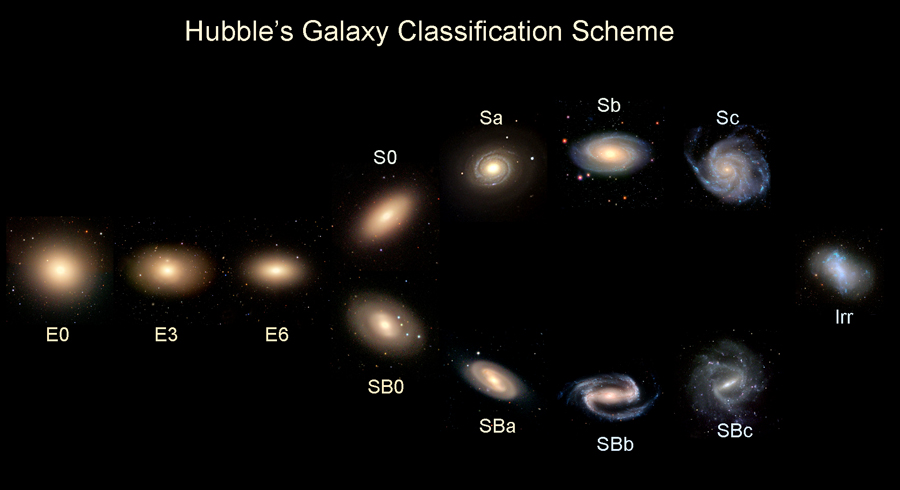
\includegraphics[width=0.6\textwidth]{Figures/HubbleTuningFork2w.jpg}
    \caption{The Hubble Tuning Fork classification scheme \citep{hubblegzdiagram}, illustrating the morphological split between Elliptical, Lenticular and Spiral galaxies.}
    \label{fig:htuningdiagram}
\end{figure}\\

On the left hand side of Figure \ref{fig:htuningdiagram} are Elliptical galaxies, characterised by their smooth, elliptical shape. Although initially thought to be a precursor to the Spiral galaxy, these galaxies tend to be older \citep{SANDAGEMountWilson} with lower rates of star formation, and lower levels of dust present. Their classification is dependent on their ellipticity, with a range between E0-E7, where the number is determined by Equation \ref{eq:elliptical}.
\begin{equation}
    e = 10 \times (1 - \frac{b}{a})
    \label{eq:elliptical}
\end{equation}
where $e$ is the ellipticity (how much it differs from being spherical in shape), $b$ is the length of the semi-minor axis, and $a$ is the length of the semi-major axis.\\

The next category of galaxies are the Lenticulars, an intermediate class between the Elliptical and Spiral classes. They serve as a transition class with a flatter form than the E7 galaxies, but no sign of bars or spiral structure \citep{SANDAGEMountWilson}. Containing mainly Population II stars (older than Population I stars, younger than Population III stars), it is thought they evolved much like Ellipticals by forming most of their stars early in their lives and then settling into a passive life from there \citep{GribbinJohn2008Gavs}. \\

Spiral galaxies form the next class in the scheme and are considered to be more structurally complex compared to Ellipticals or Lenticulars. They are characterised by their spiral arms, and are split into 3 sub-classes along the ‘Tuning Fork’, Sa, Sb, and Sc. This classification is dependent on the tightness of their spiral arms and classically the brightness of the central nucleus \citep{AGNThesis2016}. However a more recent paper \citep{Masters2019} has demonstrated the weakness of the link between the tightness of the spiral arms and the brightness of the central nucleus, showing how although this is a widely used classification scheme, it still has drawbacks. Spiral galaxies are also split into 2 sub-classes relating to the presence of the bar in the galaxy. A bar is a structure in the centre of the galaxy from which arms can originate and is crucial in investigating the formation and evolution of galaxies \citep{Sellwood_1993}. If a galaxy has a bar present it is given the classification Sb(a/b/c), those without one present are given the classification S(a/b/c).\\

The arms of Spiral galaxies are another active area of research, to better understand how they have formed as well as investigating the intense regions of star formation present. The arms themselves can be split into two general types, ‘grand design’ and ‘flocculent’ \citep{Elmegreen2014}. Grand design arms are the large scale ones typically well-defined and clear in images. They are believed to have been formed from density perturbations in the spiral structure, resulting in ‘waves’ that travel around the galaxy to form these large spiral arms. Flocculent arms are smaller, less defined arms believed to form from shock waves from supernovae that propagate through the spiral structure, creating these discontinuous arms.\\

The final class of galaxies are the Irregulars, named due to their irregular shape and lack of structure or symmetries. They are another active area of research to understand how they formed and why they have no structure unlike other classes \citep{SANDAGEMountWilson}. One form of Irregular galaxies, the Dwarf Irregulars, are important objects in understanding the evolution of higher mass galaxies due to their abundance and their diversity across the local volume our galaxy occupies \citep{dwarfgalaxies2014}.\\

All of these Hubble classes can be quantified into a numerical index (the T-Type value), with values running from -6 to 10 or 11 depending on the classification. Elliptical and Lenticular galaxies are quantified by negative values and Spiral galaxies form the majority of positive values, apart from the final values which correspond to Irregular galaxies, as shown in Table \ref{table:ttypes} \citep{1974IAUS...58....1D}.

\begin{table}[t]

\centering
\resizebox{\columnwidth}{!}{
\begin{tabular}{|c|l|l|l|l|l|l|l|l|l|l|l|l|l|l|l|l|l|}
\hline
Type T                                                   & -6                            & -5                         & -4                            & -3                            & -2                         & -1                            & 0                         & 1                       & 2                        & 3                       & 4                        & 5                       & 6                        & 7                       & 8                        & 9                       & 10                      \\ \hline
\begin{tabular}[c]{@{}c@{}}Hubble \\ Class\end{tabular} & \multicolumn{1}{c|}{$E^{-1}$} & \multicolumn{1}{c|}{$E^0$} & \multicolumn{1}{c|}{$E^{+1}$} & \multicolumn{1}{c|}{$L^{+1}$} & \multicolumn{1}{c|}{$L^0$} & \multicolumn{1}{c|}{$L^{-1}$} & \multicolumn{1}{c|}{S0/a} & \multicolumn{1}{c|}{Sa} & \multicolumn{1}{c|}{Sab} & \multicolumn{1}{c|}{Sb} & \multicolumn{1}{c|}{Sbc} & \multicolumn{1}{c|}{Sc} & \multicolumn{1}{c|}{Scd} & \multicolumn{1}{c|}{Sd} & \multicolumn{1}{c|}{Sdm} & \multicolumn{1}{c|}{Sm} & \multicolumn{1}{c|}{Im} \\ \hline
\end{tabular}
}

\caption{The conversion between the Hubble class and the T-Type value \label{table:ttypes}}
\end{table}

\subsection{Deep Learning}\label{sec:deepbackground} 
Deep learning is a form of machine learning based on artificial neural networks that have a ‘deep’ network architecture which represent different levels of a feature at different levels of the network. They are used widely across a variety of fields, from self-driving cars, medical image processing, natural language processing and much more. This is due to their ability to break down more complex features by translating simpler features at initial layers to more abstract features further into the network \citep{Lecun2015}. 
In this section I will explain some of the features of neural networks that contribute to the overall performance. 
\subsubsection{Hyperparameters} \label{sec:hyperdeep}
Hyperparameters are parameters that are set prior to training and remain constant throughout. The correct selection of them is extremely important in order to achieve a good final network performance and to train the network in a realistic time \citep{SmithHyperparameters}. These hyperparameters include the batch size, learning rate, number of epochs, activation functions, optimiser, and architecture (number of layers, layer size).\\

During training, images are loaded into batches set by the batch size and are passed through the network. One epoch is when all images in the training set have passed through the network once, and this process repeats a set amount of times, the number of epochs. Neural networks are sensitive to both of these parameters, as images loaded in larger batches tend to reach a local minimum faster and do not reach the global minimum of the loss function. Neural networks approach this global minimum with more epochs, however once it has reached this point it is necessary that the network stops training so it is less computationally expensive.\\

The architecture itself is chosen for the task, as simpler images do not require a complex network but more complex images need a suitably complex network. The number of layers affects the size of the layers, as a smaller network will need large layers earlier on so to reduce the dimensions of the vector being passed through to the classifying layers, to reduce overall run time \citep{Goodfellow-et-al-2016}.\\

Hyperparameters like the activation function and optimiser are functions chosen prior to training and directly relate to the training of the network. In a neural network each layer has weights and biases, both of which are initialised prior to training and during the training process are optimised. As seen in Equation \ref{eq:network_layer}, the input to the layer $n$, $x_{n-1}$ is multiplied by the layer weight $W_n$ and then added to the bias $b_n$. All of this is then a function of the activation function $f$, to get the final output of the layer $x_n$.
\begin{equation}
    x_n = f(W_n x_{n-1} + b_n)
    \label{eq:network_layer}
\end{equation}
\begin{figure}
    \centering
    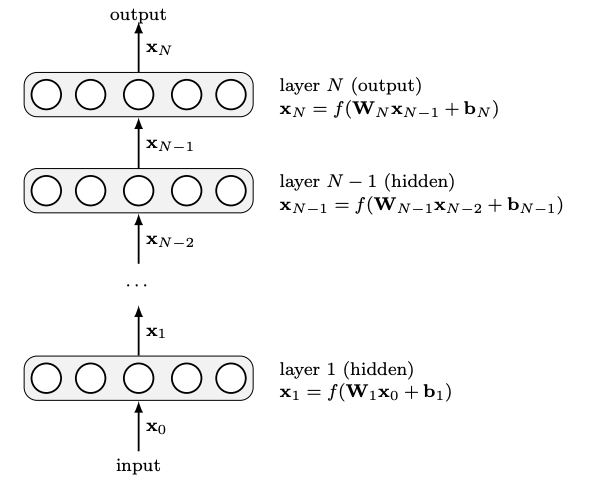
\includegraphics[width=\linewidth]{Figures/feed_forward_network.png}
    \caption{A simplified example of a neural network, with the layers and their weights and biases calculated at each step \citep{DielemanS2015}.}
    \label{fig:feed_forward}
\end{figure}
The activation function tells a neuron in a network whether it should fire or not, depending on its input. The one used in this project is a non-linear function, the rectified linear unit (ReLU), defined below in Equation \ref{eq:relu}, and outputs 0 if the input is less than or equal to 0, and then outputs the input if said input is greater than 0 \citep{Geron2017}.
\begin{equation}\label{eq:relu}
    f_{relu}(x_i) = max(0,x_i)
\end{equation}

The optimiser is another important hyperparameter. Used during training, it is this function that computes the error gradient with respect to the weights and biases during back-propagation, and then alters these to an optimum value. The learning rate is applied to the optimiser, when the optimiser alters the weights and biases. A larger learning rate alters these values more, though this can cause the optimum values to be missed.

Early examples of optimisers include the Stochastic Gradient Descent(SGD) which randomises the data being inputted, and then instead of selecting a whole data set during each training iteration it picks one data point and calculates the gradient. This speeds up computation time when compared to simpler gradient descent algorithms, as it does not sample the whole dataset on each iteration \citep{Bottou10large-scalemachine}.

The optimiser used in this project has been Adamax (Adaptive moment), an adaptive learning rate algorithm that calculates the gradient and then uses this gradient to scale the learning rate \citep{adam}.

\subsubsection{Training}\label{sec:trainingdeep}
In order to learn features and classify them into the different categories, it is first necessary to train the network on the labelled target data that you wish to classify. This is done using the back-propagation algorithm, otherwise known as the generalised delta rule \citep{KhanSalman2018AGtC}. Named after how it propagates the error back from the output through the network, this algorithm first works by inputting the first instance of training data into the network, which if it is an image can be thought of as a matrix of values. For example with the MNIST image shown in Figure \ref{fig:mnist_44} if the white pixels are assigned a value of 1 and black pixels a value of 0 then this image is simply a matrix of values between 1 and 0. For images in colour, this is simply 3 matrices of red, green and blue. 


\begin{figure}
    \centering
    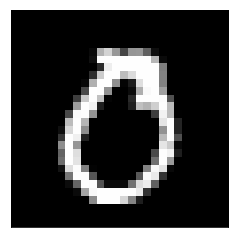
\includegraphics[width=0.5\linewidth]{Figures/MNIST_44_0.png}
    \caption{Image 44 from the MNIST database, showing a handwritten 0 \citep{lecun-mnisthandwrittendigit-2010}. When the white pixels are assigned a value of 1 and the black pixels a value of 0, this becomes a matrix containing values between 0 and 1. }
    \label{fig:mnist_44}
\end{figure}



Once this matrix of values is inputted into the network, the output from every layer is computed and the overall output error is calculated. This is done by measuring the difference between the desired output of the network and the actual output, usually in probabilities \citep{rumelhart1986}. The next step is computing how much the final layer contributed to the output error, and then the contributions to this error from the previous are computed, and so on until this error has been propagated back through the network. This pass through the network also calculates the gradient of the error with respect to the weights and biases, and this gradient is used to adjust all the weights and biases in the network. As shown in Figure \ref{fig:grad_learn}, the algorithm adjusts the weights and biases in the opposite direction of the positive gradient, moving towards the global minimum. Not all training is as simple as this; it is more normal for there to be local minima that the network can get stuck in and optimising the hyperparameters can help overcome this issue, as discussed in Section \ref{sec:hyperdeep}.

\begin{figure}
    \centering
    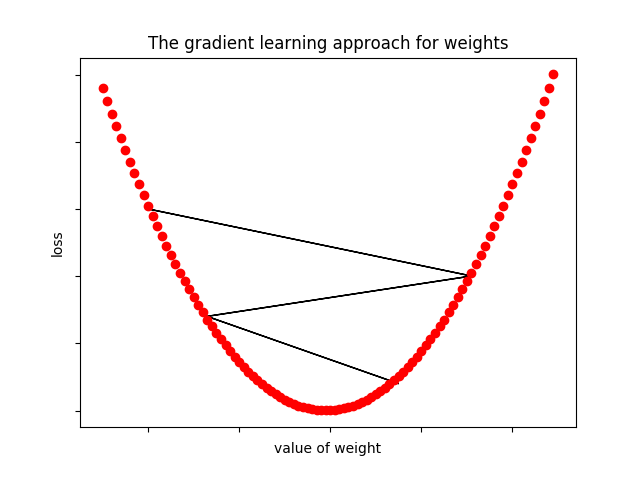
\includegraphics[width=0.7\linewidth]{Figures/gradient_learning.png}
    \caption{The gradient learning approach for the weights in the back-propagation algorithm. The curve represents the loss against the weight, and the lowest point is the optimum value for both. The straight line represents the changes made by the algorithm to optimise these values.}
    \label{fig:grad_learn}
\end{figure}
    
This process is repeated for all training data, adjusting the weights and biases until they are ideally optimised for this set of images. 

\subsubsection{Assessing the Network}\label{sec:testing}
In order to analyse how effective a network has been compared to other networks, a method of testing must be introduced that compares them the same way. As well as measuring the Accuracy and Loss for each network, the method used within this report is the Receiver Operating Characteristic curve (ROC curve), which is a plot of the True Positive Rate (TPR) against the False Positive Rate (FPR). For this example there are only two results that a classification can have, a positive classification or a negative one. 

This classification can either be True (correct) or False (incorrect), thus there are four variables which are passed to the TPR (shown below in Equation \ref{eq:tpr}) and FPR (shown below in Equation \ref{eq:fpr}), the True Positives, True Negatives, False Positives, and False Negatives. 

\begin{multicols}{2}
\begin{equation}\label{eq:tpr}
   TPR = \frac{TP}{(TP + FN)}
\end{equation}\break
\begin{equation}\label{eq:fpr}
  FPR = \frac{FP}{(TN + FP)}
\end{equation}
\end{multicols}

The ROC curve is a plot of the $TPR$ against the $FPR$, and a good classifier is a curve that occupies the upper left hand corner of the graph and has a high area under the curve. A linear line through the origin is a random classifier and is seen as the baseline \citep{FAWCETT2006861}. 

Figure \ref{fig:fmnistroc} shows two ROC curves, one of a network trained on just 10 images and another trained on 10\,000. In this example the network trained on just 10 images performs poorly and produces a ROC curve that illustrates this, demonstrating it is worse than a random classifier. However Figure \ref{fig:roc_2} represents a network that performs exceptionally well, classifying the images in the dataset almost perfectly, as demonstrated by the curve that reaches far into the upper left hand corner of the graph.


This is widely used in literature (\cite{sancheztransfer}, \cite{ackerman2018}, \cite{2018arXiv180710406D}) and will serve as our testing method to compare the 7 different tests presented.


\subsubsection{Regularisation}\label{sec:reguldeep}
When training a network on a small dataset it is possible that the network will overfit to this data, when it ‘memorises’ the dataset and achieves a high accuracy, however when it is applied to new data it does not perform well. For example when a network is trained on just 10 images from the fashion\_MNIST dataset, and then applied to 2\,800 test images it achieves an accuracy of 90\% during training, but its test accuracy is just 38\%, producing the Receiver Operating Characteristic curve (explained in Section \ref{sec:testing}) in Figure \ref{fig:roc_1}. However after training on 10\,000 images the network reached a training accuracy of 95.1\% and a final test accuracy of 89.71\%, producing the following curve in Figure \ref{fig:roc_2}. As is clear from this example, training on both datasets produces a network with a high training accuracy, however the differences become apparent when applied to new images. The network trained on fewer images does not generalise well at all and performs considerably worse than a random classifier. the network trained on the larger dataset has been exposed to a greater array of images and thus generalises very well to new data, performing as an almost perfect classifier. 
\begin{figure}[h]
\centering
    \begin{subfigure}{0.45\textwidth}
    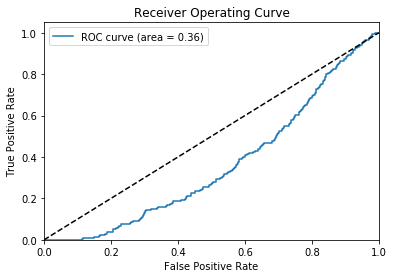
\includegraphics[width=\linewidth]{Figures/ROC2.png}
    \caption{ROC curve produced after training on a dataset of 10 images.}
    \label{fig:roc_1}
    \end{subfigure}
    \begin{subfigure}{0.45\textwidth}
    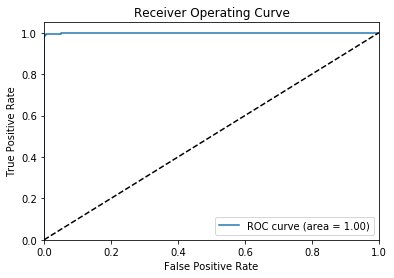
\includegraphics[width=\linewidth]{Figures/ROC2_2.png}
    \caption{ROC curve produced after training on a dataset of 10000 images.}
    \label{fig:roc_2}
    \end{subfigure}
    \caption{ROC curves for networks trained on two different sized datasets to illustrate how a network can perform well during testing but not generalise well to new data.}
    \label{fig:fmnistroc}
\end{figure}


This example shows the effects of overfitting, which is also well characterised in Figure \ref{fig:regular}. Here the network underfits to the data in the first graph, fits well to it in the second and then memorises and overfits to the data in the final graph. 

\begin{figure}[h]
    \centering
    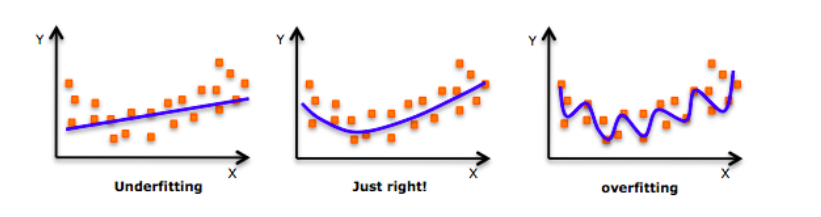
\includegraphics[width=\linewidth]{Figures/regularisation.png}
    \caption{The first graph shows an example of underfitting to the data, the second an example of fitting well to the data and the third shows an example of overfitting to the data \citep{shubham_2018}}
    \label{fig:regular}
\end{figure}

It is extremely important for a network to be able to generalise well to new data, especially in the field of identifying morphology, where there exists diverse and vast collections of galaxies, each with its own unique features. Any network applied to images of galaxies therefore has methods of regularisation (allowing it to generalise) utilised.\\

The methods of generalisation used within this paper are the application of data augmentation, and the use of dropout layers. Data augmentation is the technique of creating copies of the input data that has been transformed in some way, either by rotating, flipping, cropping, scaling etc. \citep{KhanSalman2018AGtC}. This can either serve to create a more robust network that has seen a diverse dataset of images, or it can be used to expand a smaller dataset with images that are slightly different. An example of the transformations applied to images of galaxies is shown in figure \ref{fig:dataug}.
\begin{figure}[h] 

  \begin{subfigure}[b]{0.5\linewidth}
    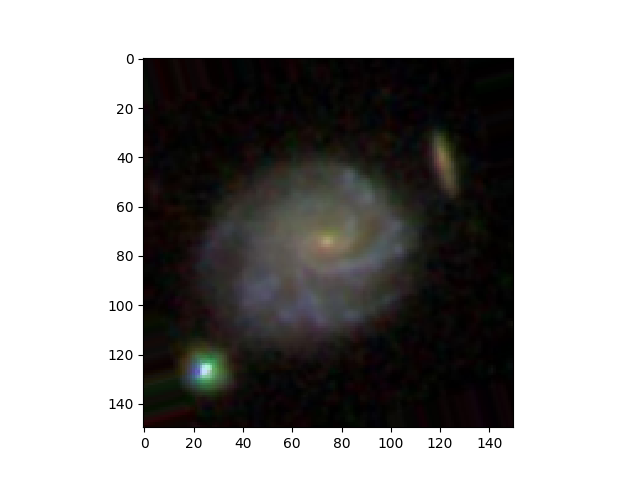
\includegraphics[width=\linewidth]{Figures/without_aug.png} 
    \caption{Original Image} \label{fig:dataug1}
  \end{subfigure} 
  \begin{subfigure}[b]{0.5\linewidth}
    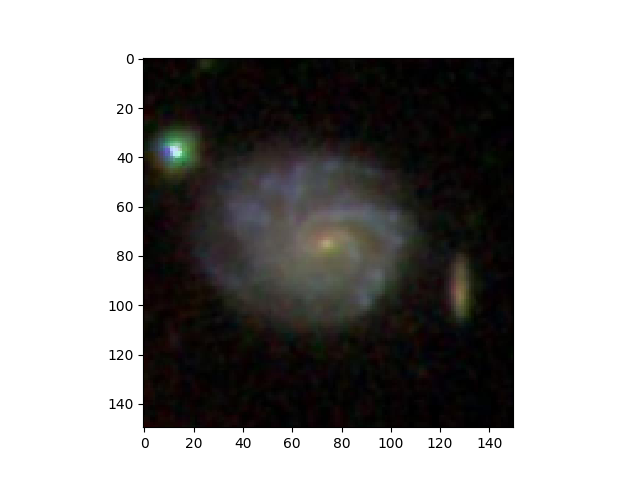
\includegraphics[width=\linewidth]{Figures/rot_aug.png} 
    \caption{Clockwise rotation of 30\degree} \label{fig:dataug2}
  \end{subfigure} 
  \begin{subfigure}[b]{0.5\linewidth}
    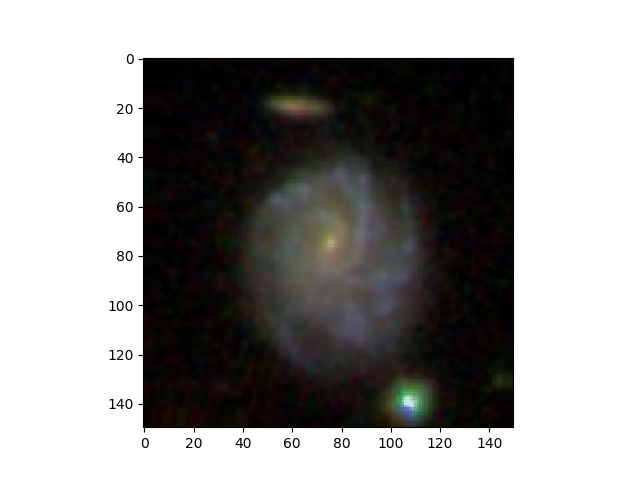
\includegraphics[width=\linewidth]{Figures/rot_2_aug.png} 
    \caption{Anticlockwise rotation of 30\degree} \label{fig:dataug3}
  \end{subfigure}
  \hfill
  \begin{subfigure}[b]{0.5\linewidth}
    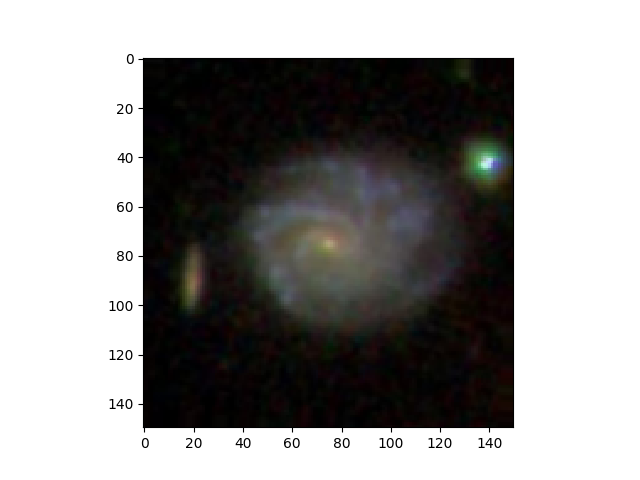
\includegraphics[width=\linewidth]{Figures/flip_aug.png} 
    \caption{Flip in the x and y axis} \label{fig:dataug4}
  \end{subfigure} 
    \caption{A series of augmentations applied to the images in the training dataset to increase the generalisation of the network by exposing it to more diverse sample of images.}
    \label{fig:dataug}
\end{figure}



The second method of regularisation is the use of dropout layers within the network. These layers randomly omit a fraction of units from the network during any training instance. This reduces the chances that any units will develop complex co-adaptions \citep{HintonG2012}, forcing each unit to be able to operate on its own without relying too heavily on other units. These layers must be used sparingly, as overuse can cause the network to lack the ability to properly learn due to the hidden units within it not working with one another. 
\newpage
\section{The Data}\label{sec:data}
In this project I pre-train networks on two separate datasets before applying them to a third dataset for testing, as well as applying them to a final dataset for comparison. For the EFIGI, Nair \& Abraham and Galaxy Zoo datasets it was necessary to transform the data into a binary form in order to simplify the training process. So for each galaxy in the samples there are three labels with values that are either 0 or 1 depending on whether it is a Spiral, Elliptical or Lenticular galaxy.

In the following sections I will discuss the properties of each dataset that was used, as well as how they were used.
\subsection{fashion\_MNIST }\label{sec:fmnistdata}
In order to explore the differences in pre-training on datasets that have no similarity to the test data, I chose the fashion\_MNIST database as it is an easily accessible set of images depicting various pieces of clothing and accessories, as well a robust classification for each image. Created to replace the MNIST database of handwritten digits, it provides a more challenging test for modern neural networks \citep{fashion_mnist}.


It is made up of 60\,000 training images and a test set of 10\,000 images, all of which are in black and white and have a label corresponding to one of the 10 classes shown in Figure \ref{fig:fashion_mnist}. 


\begin{figure}[h!]
\centering
        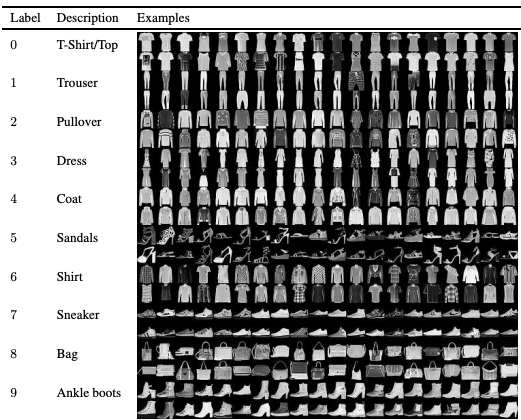
\includegraphics[width=0.7\linewidth]{Figures/fashion_mnist.png}
        \caption{An example of images from the fashion\_MNIST dataset \citep{fashion_mnist}. These images were used to pre-train a set of networks to investigate how knowledge transfers from a sample of images that are very different from the target images.}
        \label{fig:fashion_mnist}
\end{figure}
 \subsection{Nair and Abraham}\label{sec:nandabrah}
 This catalogue was created in 2010 with the goal of providing a sample of galaxies with highly detailed morphological classifications for the purpose of research into the abundances of specific morphological features, as well as a starting point for automated visual classification by image recognition algorithms \citep{nairandabraham}. It is made up of 14034 galaxies from the Sloan Digital Sky Survey Data Release 4, a highly comprehensive survey of over 6670 square degrees of the sky, imaging roughly 180 million objects \citep{sdssdr4}. The sample contains information on the presence of finer morphological features such as bars, rings and lenses, as well as the standard T-Type classification found in Table \ref{table:ttypes}.
 
 
\subsection{EFIGI}\label{sec:efigi}
The EFIGI (“Extraction de Formes Id\'{e}alis\'{e}es de
Galaxies en Imagerie”) dataset is the testing set in this project. This was used due to its size and the fact the images within the dataset are of a good quality and have a robust classification. Created in 2018, there are 4458 galaxies within the sample, all from the Sloan Digital Sky Survey Data Release 4 \citep{sdssdr4}. Each galaxy within the sample has 16 shape attributes, as well as a T-Type label which has been visually determined by 10 expert classifiers \citep{EFIGI2018}. These T-Type values match the ones found in Table \ref{table:ttypes}. 


\subsection{Galaxy Zoo}\label{sec:GZdata}
The Galaxy Zoo project is a citizen science project first launched in 2007 \citep{Lintott2008} aimed at matching the level of accuracy of expert classifiers without the time taken to do so. Volunteers create an account on the website and are then shown an image of a galaxy which they answer a series of questions on. These questions are based around the observational features of the galaxy, as shown in Figure \ref{fig:GZ_decision}. During the original project over 800\,000 images from the SDSS were classified, with an average of 38 classifications per galaxy, producing some of the largest labelled catalogues from the SDSS \citep{2011MNRAS.410..166L}. This dataset has gone on to be used in a many different papers and has shown itself to be a robust and reliable catalogue \citep{greenpeasgz, unwindinggz, barsgz, barsenvgz}.


I used data from the latest iteration of the project, Galaxy Zoo 2 \citep{Willett2013}, as a confirmation set to observe how my network classified images compared to the classifications given by volunteers. The classifications provided by volunteers have again been binarised based off the Hubble classification that was assigned. 
\begin{figure}
    \centering
    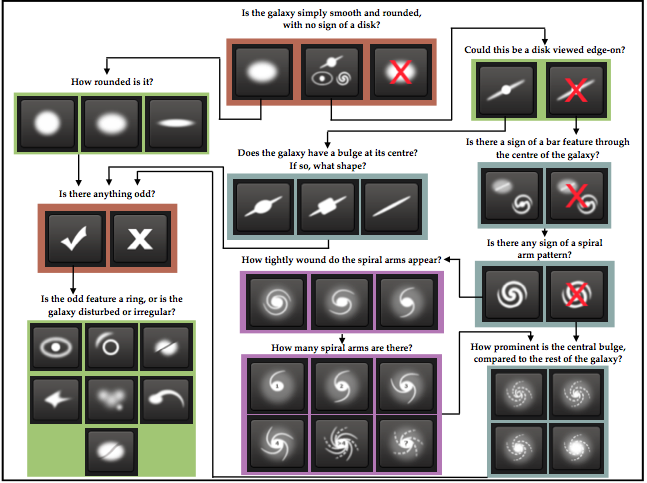
\includegraphics[width= 0.85\textwidth]{Figures/GZ_Decison_Tree.png}
    \caption{The decision tree of questions posed to volunteers as part of the Galaxy Zoo project \citep{Willett2013}. In the GZ2 catalogue, each question in the tree has an array of answers that each have a probability associated with them.}
    \label{fig:GZ_decision}
\end{figure}



\newpage
\section{Methods and Networks} \label{sec:MethodsandNetworks}
In this Section I will build upon the basic ideas presented in Section \ref{sec:deepbackground}. In Section \ref{sec:CNNdeep} I will discuss the Convolutional Neural Network, the form of neural network used within this project. Finally in Section \ref{sec:transferdeep} the method I implemented to improve the generalisation and accuracy of the network, transfer learning, will be introduced and I will elaborate on how it was used within testing.



\subsection{Convolutional Neural Networks} \label{sec:CNNdeep}
This form of neural network, CNN (convolutional neural network), was influenced by research into the visual cortex of mammals, specifically cats \citep{Hubel1959}. It was observed that neurons in the visual cortex had small receptive fields, and that they were arranged in layers from ‘simple’ to ‘complex’ cells \citep{Hubel1968}. These simpler cells identified the more generic features like horizontal lines, and then the complex cells reacted to the patterns outputted by these simpler cells to identify more abstract shapes in the images. This theory was applied to the first example of a CNN, the Neocognitron \citep{Fukushima1980}, which was constructed of many simple and complex layers to extract the lower level features, and then from these more abstract higher level features. In this Section I will discuss the general components of a CNN, as well as the specific architecture and hyperparameters used for this project.

\subsubsection{Features and Classifiers}\label{sec:featandclass}
The main aim of any deep neural network is to successfully extract relevant features from the object and then classify based off these features. Therefore the role of feature extraction and classifying layers in the neural network is unparalleled \citep{pythonmachinelearningbook}. A network is comprised of layers of these feature detectors and classifiers, arranged in certain architectures that will be explained further in Section \ref{sec:deeparchit}. \\

In a CNN the convolutional layers are the feature extractors, outputting a final abstract shape for the dense layers to classify. They carry this out so successfully by applying local receptive fields to the units, so that the first layer ‘views’ the image with a multitude of units that only ‘look’ at a series of overlapping fields. The inputs to the units from these small local fields are then quantified and outputted to a collection of units in the next layer. This means that not all units between are connected, however the network also shares weights between units in layers, as elementary features in one part of an image are likely present across the image \citep{Lecun1998}. \\

As discussed above, the theory behind this neural network is to extract lower level features early in the network and then from these extract the higher level features. Once these higher level features have been extracted, they then are passed to the classifier layers, otherwise known as fully-connected layers. These are the layers that will output the classes or probabilities, depending on the problem presented to the network and the activation function used. These fully-connected layers are named as such due to each unit in the layer being connected to every unit in the previous layer, and when the number of units is set to the desired number of answers (e.g. for  binary cases this is 1 output) the output vector is a probability that related whether each image is in a certain class. \\

For example when testing on the fashion\_MNIST database there are 10 classes an image could fall into, from a t-shirt to a coat. The final layer in the network trained on these images has 10 units in, meaning it outputs 10 values corresponding to those 10 classes, as shown in Figure \ref{fig:fmnistpredict}.\\
\begin{figure}
    \centering
    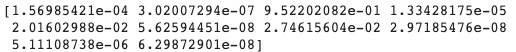
\includegraphics[width=0.8\linewidth]{Figures/fashion_mnist_outputs.png}
    \caption{Some predictions for images from the fashion\_MNIST dataset, with the values inside each square bracket belonging to one of 10 probabilities per image.}
    \label{fig:fmnistpredict}
\end{figure}


The fully-connected layer also consists of an activation function which takes a vector of real numbers and outputs a probability distribution relating to the actual function itself. In the network explained in Section \ref{sec:deeparchit}, the activation function used in this final layer is the softmax function, which has the purpose of highlighting the highest values in the vector and suppressing those values which are significantly lower \citep{Bishop:998831}. Going back to the fashion\_MNIST example, in the series of values in the square brackets clearly the value, $9.77\times10^{-1}$, is the value closest to 1 and the image belongs to whichever class that corresponds to.



\subsubsection{Pooling Layer}
Once the lower level features have been extracted, the specific location of these features relative to the image are less important and could even be potentially harmful to training as these features will not occur in the same place for all images \citep{Lecun1998}. What is important is the location of features relative to other features, as well as the more abstract patterns that can be extracted from the outputs from lower layers. In order to extract these features, pooling layers are put in to effectively down-sample the image and make higher level features easier for the network to identify by lowering the resolution.\\

Figure  \ref{fig:poolingexample2} shows the visualisation of one of the pooling layers for an image (Figure \ref{fig:testimage}) passed through the network trained on the Nair \& Abraham dataset. Focusing on the lighter yellow elements of each sub image in the grid, as the images are passed from the previous layer in the network to this pooling layer, the resolution of each sub image is reduced. The spiral features become more prominent, meaning that the next convolutional layer can identify the higher level patterns and better classify the image.

\begin{figure}
    \centering
    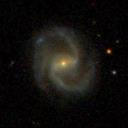
\includegraphics[scale=1]{Figures/10249.jpg}
    \caption{The image passed through the network when plotting visualisations of each network layer}
    \label{fig:testimage}
\end{figure}

\begin{figure}[h]
    \centering
    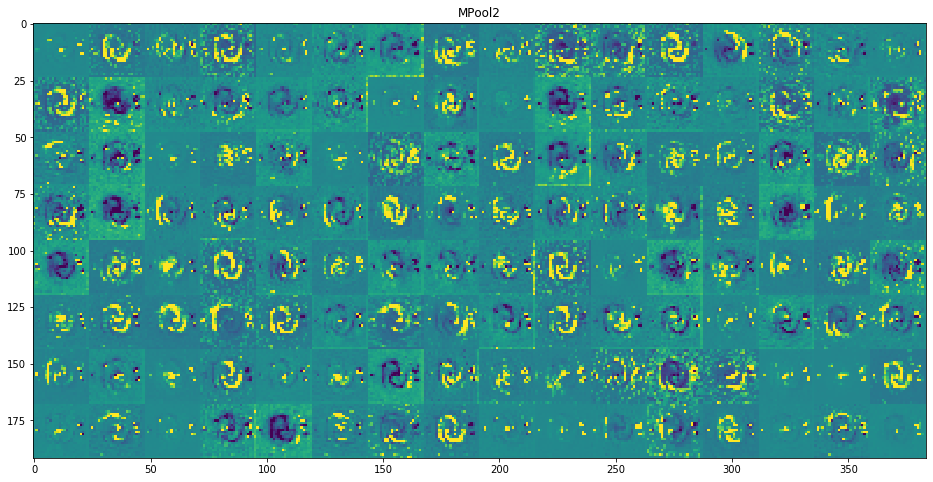
\includegraphics[width=0.9\linewidth, trim={3.3cm 4.5cm 4.1cm 4.5cm}, clip]{Figures/activation_layers/Mpool_2.png}
    \caption{A selection of visualisations from the Max Pooling layer used in the network described in Section \ref{sec:deeparchit}. The yellow elements in the images represent what this layer in the network ‘looks’ at when exposed to the image. The lower resolution generated by the Max Pooling layer allows for the spiral structure to be highlighted.}
    \label{fig:poolingexample2}
\end{figure}
\subsubsection{Network Architecture}\label{sec:deeparchit}
\begin{figure}
    \centering
    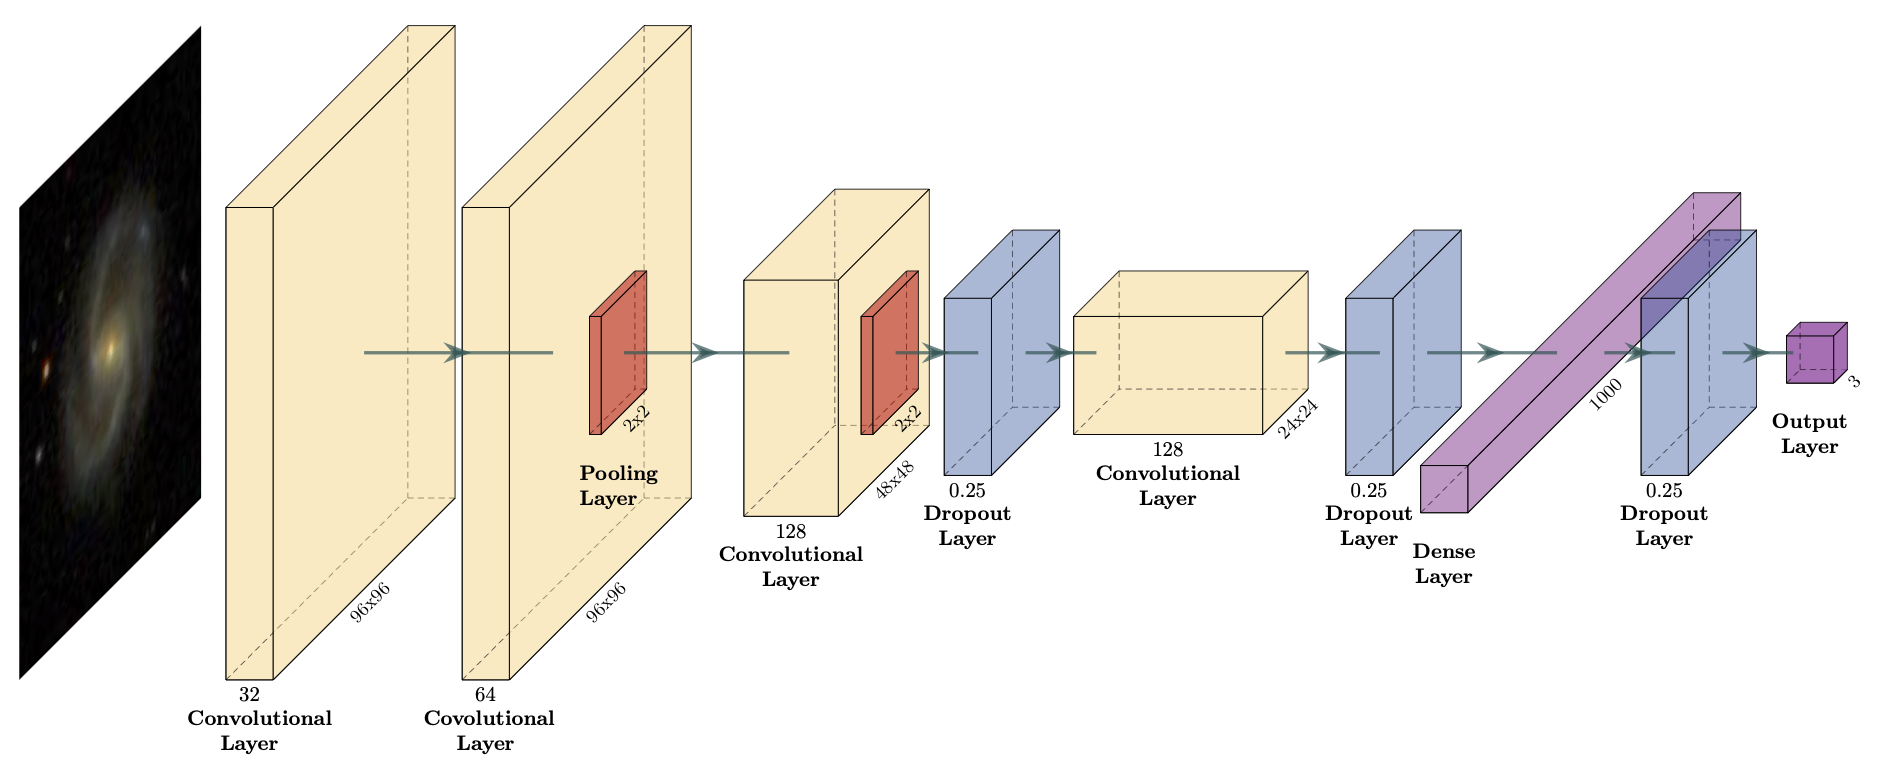
\includegraphics[width=1.\linewidth]{Figures/net_arc.png}
    \caption{The network architecture used within this project}
    \label{fig:netarch}
\end{figure}
Within this project a variety of networks were considered, but due to its success in classifying galaxies by morphology \citep{DielemanS2015,2015ApJS..221....8H,2018arXiv180710406D} the convolutional neural network discussed above was used. More specifically an adapted version of the one used in \cite{sancheztransfer} was applied to this dataset and was used in each test that was carried out. It was adapted to fit the dataset and the outputs that were required, as well as some small adjustments to filter sizes and dropout layers to increase accuracy. This was carried out using the \verb|KERAS| \citep{chollet2015keras} library, a high level neural network API that runs on top of the \verb|TensorFlow| framework.\\

The images were inputted to the network with shape (96,96,3), downsized from their original downloaded size of (424,424) in order to reduced computational cost and overfitting. The 3 represents the RGB format they were used in, as an analysis of the images showed that there did not seem to be any dependence between classes on the colour of the galaxy.\\

The network architecture, shown in Figure \ref{fig:netarch}, consists of four convolutional layers with the leaky ReLU activation function, as well as two MaxPooling2D layers and then finished with two dense layers. The convolutional layers have different filter sizes of (6x6), (5x5), (2x2) and (3x3) respectively, and the MaxPooling2D layers (with pooling sizes of 2x2) follow the second and third convolutional layers. Initially, unlike the original network found in \cite{sancheztransfer}, dropout was only carried out after the second MaxPooling2D layer as accuracy was better however, the network did not generalise well to new data so the other two dropout layers were added back in.

The first fully-connected layer has 1000 units, which was found to perform optimally despite not being fully-connected to every unit in the previous layer, as this would have had too high a computational cost. The final dense layer has just 3 units, to account for the 3 classes an image can belong to for our data, meaning the network outputs 3 probabilities for each image it is shown. \\

This network trained on 32 images in a batch, as increasing or decreasing this value was found to increase computational cost and greatly increase the loss. It was then trained over 15 epochs for the pre-trained networks and 10 epochs for the fine-tuned. The network was found to converge after about 8 or 9 epochs and then fluctuated around a value for the final epochs.



\subsection{Transfer Learning}\label{sec:transferdeep}
In the field of classification of galaxies by their morphology, datasets tend to be quite large \citep{dr14sdss}. However, when it comes to identifying some of the finer features of galaxies such as the number of spiral arms, if a galaxy is edge on, or if a ring is present within the galaxy, the datasets are relatively small in comparison. As discussed earlier in Section \ref{sec:reguldeep}, networks trained on smaller datasets can overfit to the data and not perform well when applied to new data. Although various techniques can be applied to improve this generalisation, they can sometimes have the negative effect of lowering the accuracy (with dropout layers), so other techniques must be applied to aid in regularisation.\\

Transfer learning is the process of pre-training a network on one dataset, and then carrying out some form of fine-tuning in order to prime the network for the target data. In the context of this project, fine-tuning refers to training certain layers after the pre-training on another dataset. This technique is still relatively new to this field, with really only one other paper \citep{sancheztransfer} having applied transfer learning to classifying galaxies by their morphologies. However in \cite{ackerman2018} a neural network was trained on ImageNet \citep{10026679837} (a collection of colour images of everyday objects) and the results showed that pre-training modestly improved how well the network generalised to the images of galaxy mergers.\\

Within this project I am looking to investigate how well a network performs when pre-trained on a dataset of very different images, and then a dataset of images similar to the target data, and to achieve this I will be using the fashion\_MNIST (Section \ref{sec:fmnistdata}) and Nair \& Abraham (NA10) (Section \ref{sec:nandabrah}) datasets. When testing on the EFIGI dataset I will be classifying galaxies into 3 classes, Lenticular, Elliptical and Spiral (further description of the data found in Section \ref{sec:efigi}). The fashion\_MNIST set contains images of pieces of clothing such as coats, bags, and shoes etc., and the NA10 set contains images of galaxies that are used to train a neural network to classify based on morphology. As well as providing different datasets I will also be looking at how varying the type of fine-tuning affects the final performance. First, I will fine-tune the final dense layers of the network, otherwise known as the classifying layers, and then I will fine-tune on a selection of layers as well as the dense ones. After pre-training and fine-tuning the networks will be applied to the EFIGI dataset to measure their performance. Table \ref{tab:transfertest} shows the different tests that will be carried out, as well as the sizes of the training and testing datasets for each test.\\




\begin{table}[]
\centering
\begin{tabular}{r|l|l|c|c|c|}
\cline{2-6}
                         & Training Dataset & Testing Dataset & No. Pre-train & No. Train & No. Test \\ \hline
\multicolumn{1}{|r|}{a)} & EFIGI      & EFIGI           & N/A           & 3000      & 758      \\ \hline
\multicolumn{1}{|r|}{b)} & fashion\_MNIST   & EFIGI           & 60000         & 0         & 4458     \\ \hline
\multicolumn{1}{|r|}{c)} & fashion\_MNIST  & \begin{tabular}[c]{@{}l@{}}EFIGI \\ (just dense layers trained)\end{tabular}     & 60000 & 3000 & 758 \\ \hline
\multicolumn{1}{|r|}{d)} & fashion\_MNIST  & \begin{tabular}[c]{@{}l@{}}EFIGI \\ (fine-tuned on multiple layers)\end{tabular} & 60000 & 3000 & 758 \\ \hline
\multicolumn{1}{|r|}{e)} & Nair \& Abraham  & EFIGI           & 10956         & 0         & 4458     \\ \hline
\multicolumn{1}{|r|}{f)} & Nair \& Abraham & \begin{tabular}[c]{@{}l@{}}EFIGI \\ (just dense layers trained)\end{tabular}     & 10956 & 3000 & 758 \\ \hline
\multicolumn{1}{|r|}{g)} & Nair \& Abraham & \begin{tabular}[c]{@{}l@{}}EFIGI \\ (fine-tuned on multiple layers)\end{tabular} & 10956 & 3000 & 758 \\ \hline
\end{tabular}
\caption{The dataset sizes for each test carried out }
\label{tab:transfertest}
\end{table}

When fine-tuning the network the ability to train is turned off for certain layers but left on for others. When investigating the visualisations of the how the layers view images that pass through the network, it became clear that to fine-tune effectively it was necessary to just fine-tune the last two convolutional layers as well as the dense ones. This stems from the fundamental theory of CNNs, that the first few layers pick up lower level features like edges and curves, whilst layers later in the network identify higher level features that are essential in classifying the image. Figure \ref{fig:fashionconv2} shows the visualisations for the second convolutional layers for the image shown in Figure \ref{fig:testimage} after being fed though the network that is pre-trained on fashion\_MNIST. \\


\begin{figure}
    \centering
    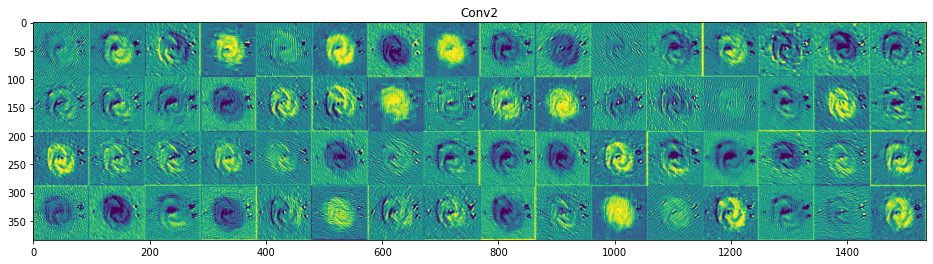
\includegraphics[width=\linewidth]{Figures/activation_layers/fashion_conv2.png}
    \caption{The visualisation for the second convolutional layer from the network pre-trained on fashion\_MNIST. Although clearly not adept at identifying the more specific features, the network still manages to identify some general features that are useful for later layers.}
    \label{fig:fashionconv2}
\end{figure}





The choice to fine-tune the last two convolutional layers comes from the analysis of the visualisations from the network pre-trained on the Nair \& Abraham dataset shown in Figures \ref{fig:naconv3} and \ref{fig:naconv4}.
\begin{figure}[b]
    \centering
    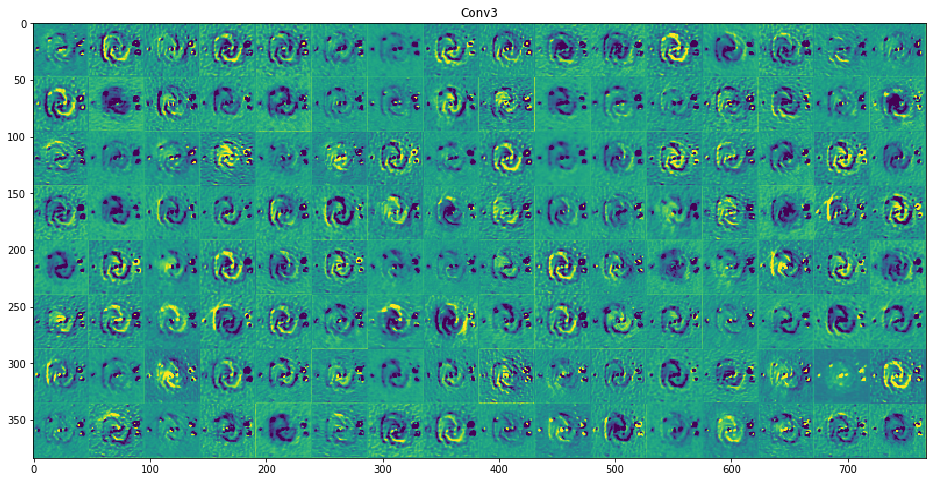
\includegraphics[width=0.8\linewidth,trim={3.3cm 4.5cm 4.1cm 4.5cm}, clip]{Figures/activation_layers/Conv3.png}
    \caption{A selection of visualisations from the third convolutional layer from the network pre-trained on the Nair \& Abraham dataset. The specific spiral features are highlighted here more clearly than in previous visualisations of layers.}
    \label{fig:naconv3}
\end{figure}
\begin{figure}[]
    \centering
    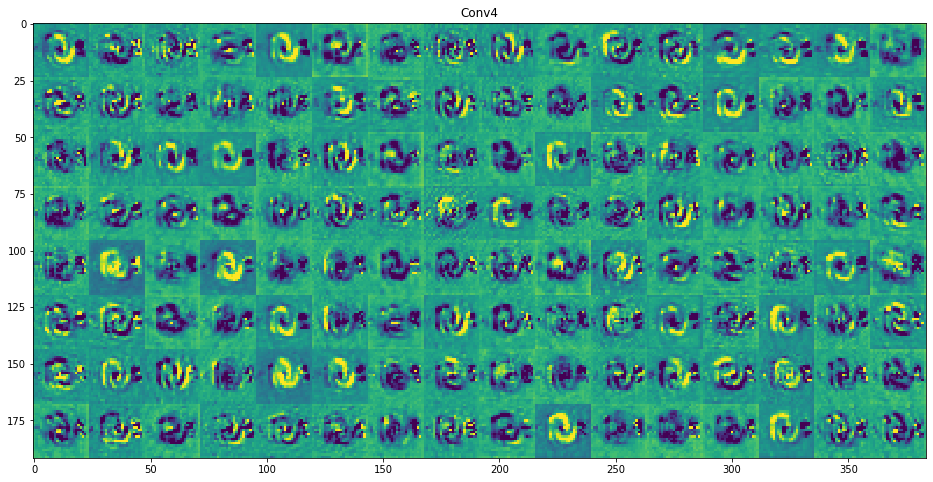
\includegraphics[width=.8\linewidth,trim={3.3cm 4.5cm 4.1cm 4.5cm}, clip]{Figures/activation_layers/Conv4.png}
    \caption{A selection of visualisations from the fourth convolutional layer from the network pre-trained on the Nair \& Abraham dataset. These lower resolution visualisations clearly show how this layer is extracting higher level features that are specific to this image. When fine-tuning this layer must be retrained in order to allow the network to adjust for a different sample of images from the one it was pre-trained on.}
    \label{fig:naconv4}
\end{figure}
The higher level spiral features are clear in these visualisations, which implies that these are the layers where the feature detection become specific for the task of galaxies. Therefore these are the two layers that will be fine-tuned in the testing as well the dense layers.


\newpage

\section{Results and Discussion}\label{sec:results}
In this Section I will lay out the results from the 7 tests carried out to analyse the effectiveness of transfer learning from different datasets, and how different types of transfer learning impact the overall performance. Below I will present the results themselves and then in Section \ref{sec:analysis} I will discuss the meaning of the results. Finally in Section \ref{sec:classified_images} I will present correctly and incorrectly classified images from the Galaxy Zoo dataset and discuss where my network had faults.


The accuracy and loss values for the test carried out are given in Table \ref{tab:results}, and in figures \ref{fig:roccurves1} and \ref{fig:roccurves2} the ROC curves for each class (Lenticular, Elliptical, Spiral) are shown. 



\begin{table}[]
\centering
\begin{tabular}{r|l|l|c|c|}
\cline{2-5}
                         & Training dataset & Testing Dataset                                                              & Accuracy & Loss  \\ \hline
\multicolumn{1}{|r|}{a)} & EFIGI            & EFIGI                                                                        & 0.853    & 0.309 \\ \hline
\multicolumn{1}{|r|}{b)} & fashion\_MNIST   & EFIGI                                                                        & 0.604    & 0.955 \\ \hline
\multicolumn{1}{|r|}{c)} & fashion\_MNIST   & \begin{tabular}[c]{@{}l@{}}EFIGI \\ (just dense layers trained)\end{tabular} & 0.736    & 4.244 \\ \hline
\multicolumn{1}{|r|}{d)} & fashion\_MNIST  & \begin{tabular}[c]{@{}l@{}}EFIGI\\ (fine-tuned on multiple layers)\end{tabular} & 0.736 & 4.244 \\ \hline
\multicolumn{1}{|r|}{e)} & Nair \& Abraham  & EFIGI                                                                        & 0.764    & 0.631 \\ \hline
\multicolumn{1}{|r|}{f)} & Nair \& Abraham  & \begin{tabular}[c]{@{}l@{}}EFIGI\\ (just dense layers trained)\end{tabular}  & 0.885    & 0.229 \\ \hline
\multicolumn{1}{|r|}{g)} & Nair \& Abraham & \begin{tabular}[c]{@{}l@{}}EFIGI\\ (fine-tuned on multiple layers)\end{tabular} & 0.936 & 0.223 \\ \hline
\end{tabular}
\caption{The accuracy and loss values for the various tests carried out}
\label{tab:results}
\end{table}



\begin{figure}[t!]
  \begin{subfigure}[t]{0.5\linewidth}
    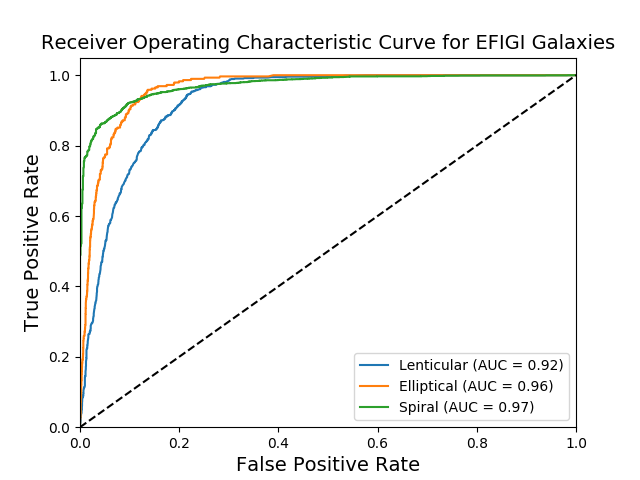
\includegraphics[width=\linewidth]{Figures/Results_ROC's/ROC_curves_E_on_E.png}
    \caption{ EFIGI on EFIGI}
    \label{fig:e_on_e}
  \end{subfigure}
  \begin{subfigure}[t]{0.5\linewidth}
    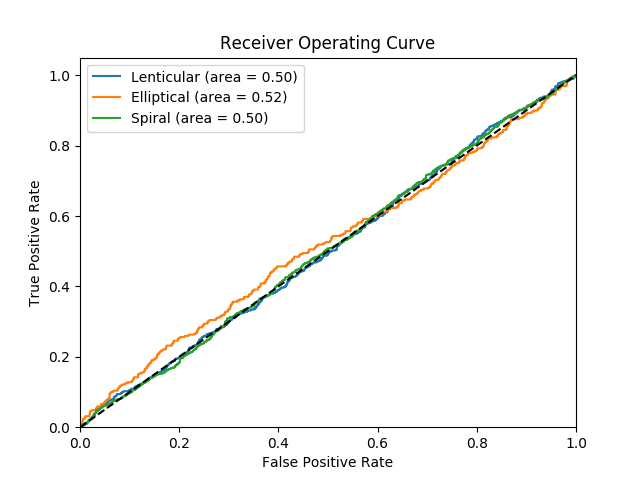
\includegraphics[width=\linewidth]{Figures/Results_ROC's/F_on_E.png} 
    \caption{ fashion\_MNIST on EFIGI} \label{fig:f_on_e}
  \end{subfigure} 
  \begin{subfigure}[t]{0.5\linewidth}
    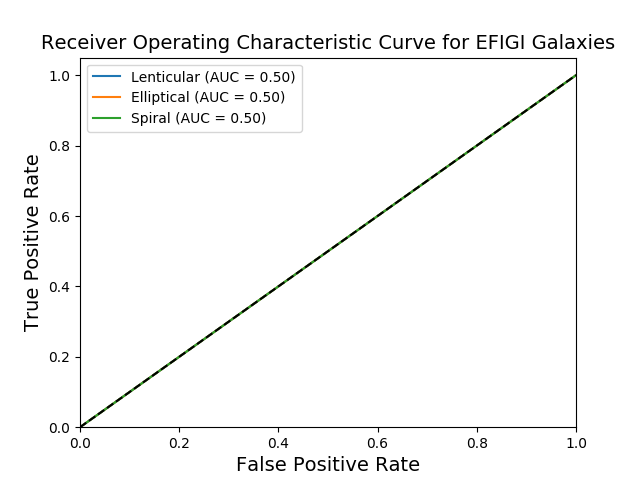
\includegraphics[width=\linewidth]{Figures/Results_ROC's/F_on_E_JD.png} 
    \caption{ fashion\_MNIST on EFIGI - just dense layers trained} \label{fig:f_on_e_JD}
  \end{subfigure} 
  \begin{subfigure}[t]{0.5\linewidth}
    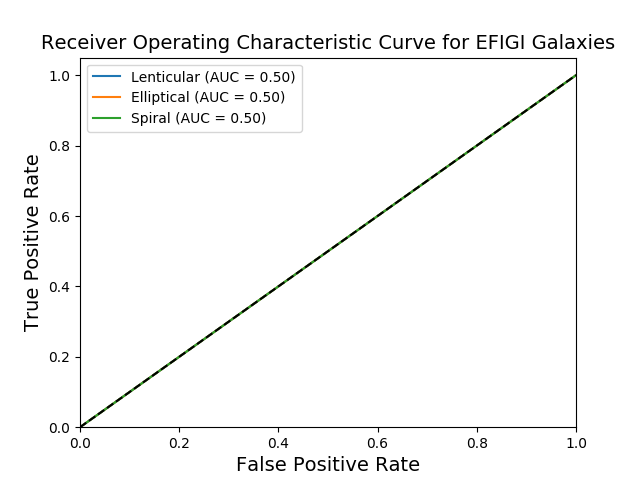
\includegraphics[width=\linewidth]{Figures/Results_ROC's/F_on_E_FTpng.png} 
    \caption{ fashion\_MNIST on EFIGI - Fine Tuning} \label{fig:f_on_e_FC}
  \end{subfigure}
  \caption{The True Positive Rate against the False Positive Rate for Tests a-d. The three separate lines represent the three classes of galaxy that each image was given a prediction for, Spiral, Elliptical and Lenticular. The dotted line depicts a random classifier. The area under the curve is given for each classification; this directly correlates with performance.}
  \label{fig:roccurves1}
\end{figure}

\begin{figure}[t!]
  \begin{subfigure}[t]{0.5\linewidth}
    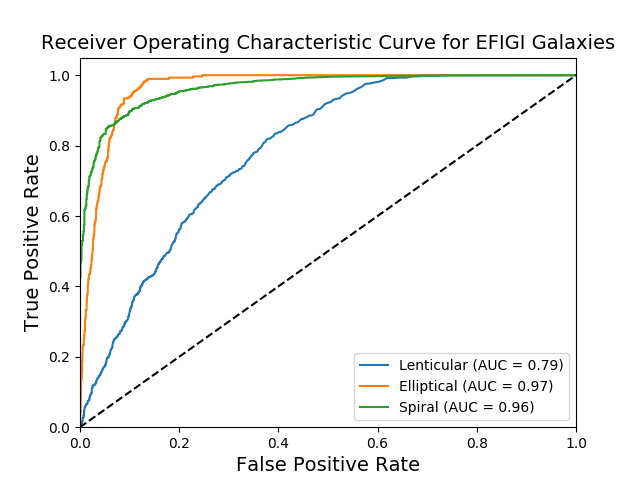
\includegraphics[width=\linewidth]{Figures/Results_ROC's/ROC_A_on_E.png} 
    \caption{ Nair \& Abraham on EFIGI} \label{fig:A_on_e}
  \end{subfigure} 
  \begin{subfigure}[t]{0.5\linewidth}
    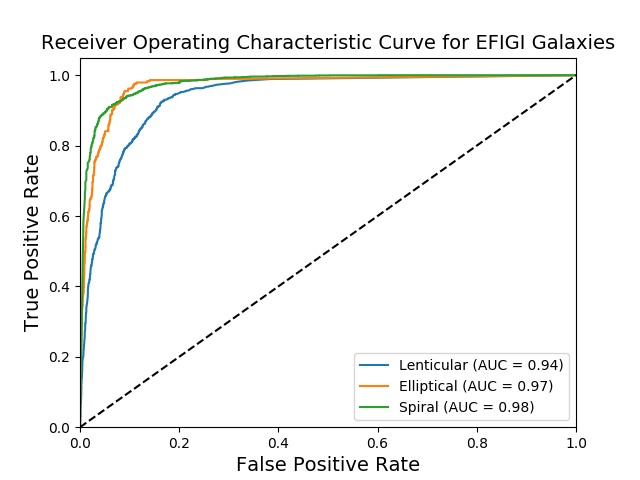
\includegraphics[width=\linewidth]{Figures/Results_ROC's/A_on_E_JD.png} 
    \caption{ Nair \& Abraham on EFIGI - just dense layers trained} \label{fig:A_on_e_JD}
  \end{subfigure} 
  \begin{center}
  \begin{subfigure}[t]{0.5\linewidth}
    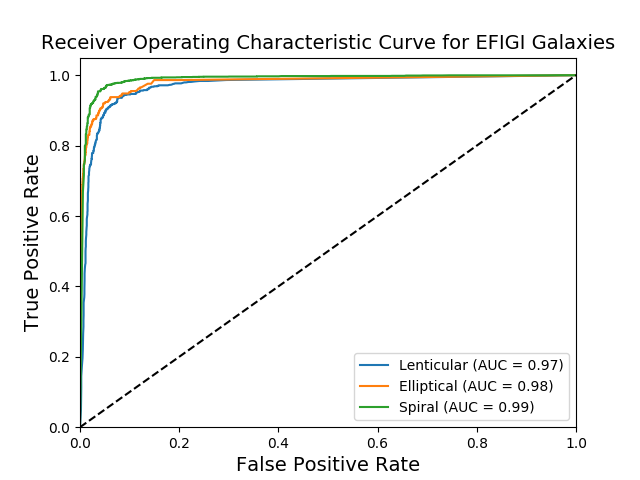
\includegraphics[width=\linewidth]{Figures/Results_ROC's/A_on_E_FT.png} 
    \caption{ Nair \& Abraham on EFIGI - Fine Tuning} \label{fig:A_on_e_FC}
  \end{subfigure}
  \end{center}
  \caption{The True Positive Rate against the False Positive Rate for Tests e-f. The three separate lines represent the three classes of galaxy that each image was given a prediction for, Spiral, Elliptical and Lenticular. The dotted line depicts a random classifier. The area under the curve is given for each classification; this directly correlates with performance.}
  \label{fig:roccurves2}
\end{figure}


\subsection{Analysis} \label{sec:analysis}
The first main result for the network trained on EFIGI data directly applied to EFIGI data gives an accuracy of $85.3\%$, which will be used as a baseline to compare the transfer learning tests against. Notably, the highest accuracy is achieved by the network pre-trained on Nair \& Abraham (NA) and then fine-tuned on multiple layers, achieving an accuracy of $93.6\%$ compared to the lowest accuracy, achieved by the fashion\_MNIST network applied to the EFIGI data with no fine-tuning, achieving an accuracy of $60.4\%$.\\

It is clear from Table \ref{tab:results} that the networks pre-trained on the NA10 network and then applied to the EFIGI data are more effective and accurate than those pre-trained on the fashion\_MNIST dataset, with the NA10 pre-trained networks achieving better accuracy on each comparative test. This could be attributed to the vast differences between these two datasets relative to the EFIGI data. The fashion\_MNIST data has no similarities to the galaxies found in the EFIGI data, as the objects have minimal curved or spiral patterns, and they have very solid outlines unlike the ellipticals and lenticulars found in EFIGI. On the other hand, the NA10 data is quite similar, with only differences in scale and colour being the notable contrasts, as seen in Figure \ref{fig:efigi/na}.

\begin{figure}[t!]
    \centering
    \begin{subfigure}[t]{0.4\linewidth}
        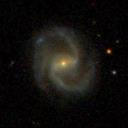
\includegraphics[width=\linewidth]{Figures/10249.jpg}
        \caption{An image from the Nair \& Abraham dataset}
    \end{subfigure}
    ~
    \begin{subfigure}[t]{0.4\linewidth}
        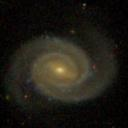
\includegraphics[width=\linewidth]{Figures/2182.jpg}
        \caption{An image from the EFIGI dataset}
    \end{subfigure}
    \caption{Images from the two datasets, see the contrasts in scale and colour between the two.}
    \label{fig:efigi/na}
\end{figure}

Also clear is that pre-training on NA10 generally gives a better result than if a network is not, provided that some form of fine-tuning takes place. This aligns with the hypothesis that pre-training improves a networks performance on a chosen task, as it initialises the network weights so they are primed for images of galaxies. \\

I also tested different fine-tuning methods within the pre-training tests, between just fine-tuning the dense layers and fine-tuning a selection of multiple layers (the choice of which layers explained in Section \ref{sec:transferdeep}). Fine-tuning multiple layers appears to be the better method, achieving better accuracies when applied to both datasets. This agrees with the theory presented above, as fine-tuning the final two convolutional layers that extract higher level features should better prepare the network for the target data. When fine tuning just the dense layers only the classifier is being adjusted for this dataset, so the feature extractor is still extracting features specific to the data it was pre-trained on. \\

The Receiver Operating Characteristic curves (ROC curves) shown in Figures \ref{fig:roccurves1} and \ref{fig:roccurves2} supports the above results that pre-training on data similar to the testing data improves the final results. As explained in Section \ref{sec:testing} a ROC curve can be used to compare networks, with a high performing network producing a curve that reaches high into the top left had corner of the graph, and a random classifier represented as a linear line. Figure \ref{fig:e_on_e} is expected for a network trained on the dataset it is being tested on, however due to the training dataset size being small this network did not perform as well as if it had been exposed to a larger dataset. 

The ROC curves presented in Figures \ref{fig:f_on_e}, \ref{fig:f_on_e_JD} and \ref{fig:f_on_e_FC} reflect the accuracy values presented in Table \ref{tab:results}, with them appearing akin to a random classifier. When investigating the predictions made by these networks it is clear why they appear to be random classifiers , as they seem to predict all images in the dataset as one particular class. This classification may be correct for some galaxies (those with that classification), meaning the accuracy is not that low. However, the ROC curve demonstrates this fault as it takes into account those galaxies that have received incorrect predictions.

In Figure \ref{fig:A_on_e}, the network is seen to perform worse than the network trained on EFIGI applied to the EFIGI data, which is expected as the NA10 data differs slightly in terms of the size of the galaxy in each image and the colour (demonstrated in Figure \ref{fig:efigi/na}). However, this network performs much better than the network pre-trained on fashion\_MNIST, which is again expected as the fashion\_MNIST data does not relate to the NA10 or EFIGI data in any way. 

The final two ROC curves in Figures \ref{fig:A_on_e_JD} and \ref{fig:A_on_e_FC} are great examples of how transfer learning has improved the overall performance of the networks when applied to data with a small training set. The network that has had just the dense layers fine-tuned on the EFIGI data outperforms the network trained on EFIGI and the one trained on NA10. The network that has had the final two convolutional layers fine-tuned as well as the dense layers is the highest performing network, which aligns well with the theory.

Across all the networks Elliptical and Spiral galaxies are seen to be more accurately classified as opposed to Lenticular galaxies, as the ROC curve is lower for each of these in each figure. This is unexpected as within both the NA10 and EFIGI datasets the number of Lenticular galaxies is higher than the number of Elliptical galaxies, so I predicted that the networks would perform better on Lenticulars. A reason for this could be that Spiral and Elliptical galaxies look quite different from one another, so the network does not have difficulty discerning between these two. However, Lenticulars are seen as the ‘intermediate’ galaxy between these two, so the network could be struggling to identify these and differentiate them from the other classes.


However, for all networks Spiral galaxies are most accurately classified, which is expected as they make up most of the data in both EFIGI and NA10 datasets.

\subsection{Classified Images} \label{sec:classified_images}
In this Section I will present correctly and incorrectly classified images from the Galaxy Zoo 2 (GZ2) dataset and using these I will highlight where the network performed well and where it had faults, as well as some potential faults in the dataset itself. The highest performing network (pre-trained on NA10 and fine-tuned over multiple layers) was used to classify 118000 images, achieving an accuracy of $45\%$, and producing the ROC curve shown in Figure \ref{fig:gz_roccurve}. This low accuracy could be down to the lower quality of the GZ2 images, as well as the network not being fine-tuned on those specific images. \\
\begin{figure}[h]
    \centering
    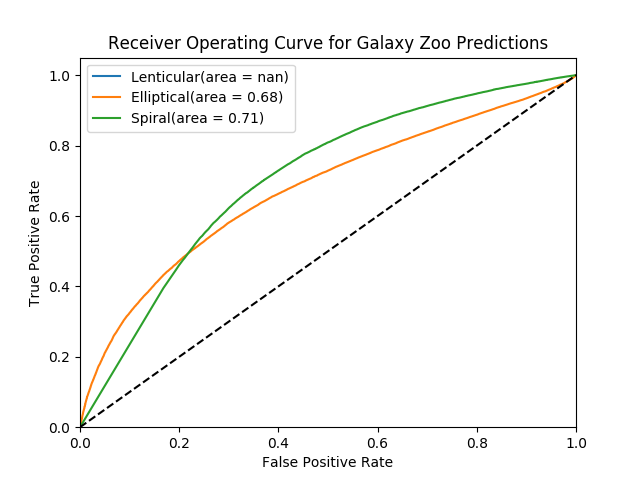
\includegraphics[width=0.6\linewidth]{Figures/GZ_predictions.png}
    \caption{The ROC curve for the predictions of images from the Galaxy Zoo 2 dataset. There is no line for the Lenticulars as no galaxies in the GZ2 dataset are classified as Lenticulars. The network does not perform as well as when applied to EFIGI data, but this is expected due to the differences in images from GZ2}
    \label{fig:gz_roccurve}
\end{figure}
\begin{figure}[h]
\centering
    \begin{subfigure}[t]{0.23\linewidth}
    \centering
    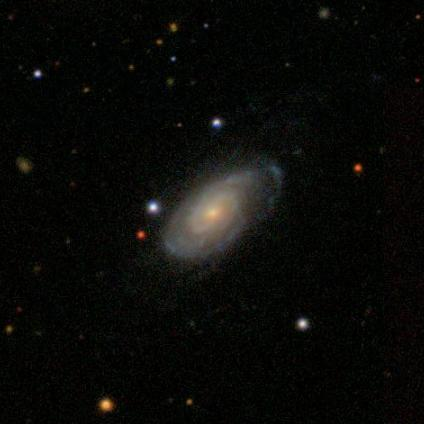
\includegraphics[width=\linewidth]{Figures/Correctly_Classified/Spiral/16.jpg}
    \caption{}
    \label{fig:correct_1}
    \end{subfigure}
    \begin{subfigure}[t]{0.23\linewidth}
    \centering
    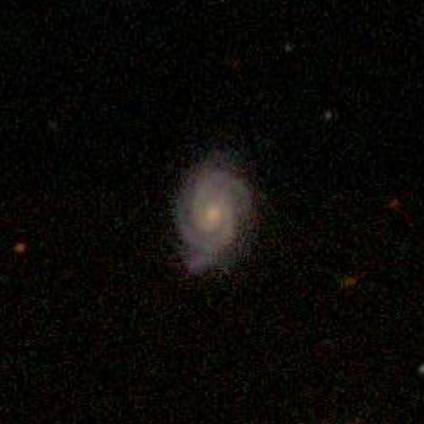
\includegraphics[width=\linewidth]{Figures/Correctly_Classified/Spiral/18.jpg}
    \caption{}
    \label{fig:correct_2}
    \end{subfigure}
    \begin{subfigure}[t]{0.23\linewidth}
    \centering
    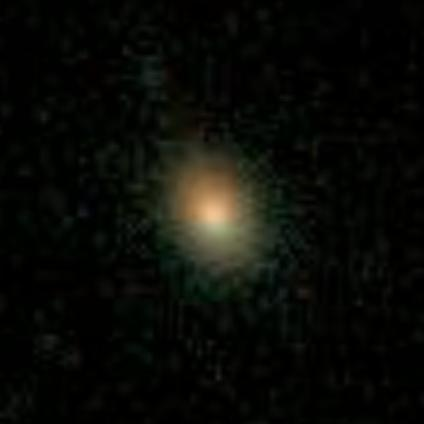
\includegraphics[width=\linewidth]{Figures/Correctly_Classified/Elliptical/157610.jpg}
    \caption{}
    \label{fig:correct_3}
    \end{subfigure}
    \begin{subfigure}[t]{0.23\linewidth}
    \centering
    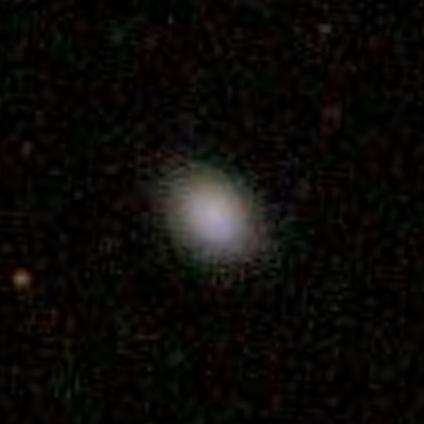
\includegraphics[width=\linewidth]{Figures/Correctly_Classified/Elliptical/110768.jpg}
    \caption{}
    \label{fig:correct_4}
    \end{subfigure}
    
    \caption{A sample of four correctly classified images from the Galaxy Zoo 2 sample \citep{Willett2013}. Figures \ref{fig:correct_1} and \ref{fig:correct_2} show two Spiral galaxies that the network correctly identified as Spirals, and then Figures \ref{fig:correct_3} and \ref{fig:correct_4} show two Elliptical galaxies the network correctly identified as Ellipticals. }
    \label{fig:correctly_classified}
\end{figure}
\begin{figure}[h]
\centering
    \begin{subfigure}[t]{0.23\linewidth}
    \centering
    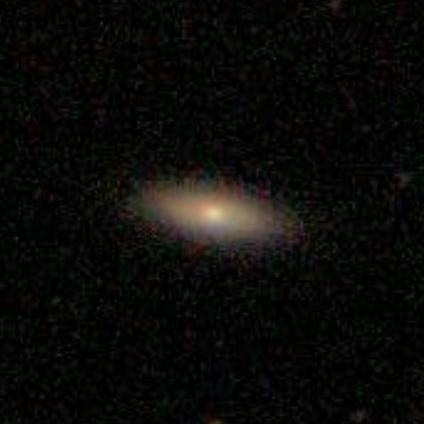
\includegraphics[width=\linewidth]{Figures/Wrongly_Classified/Lenticular/14538.jpg}
    \caption{}
    \label{fig:incorrect_1}
    \end{subfigure}
    \begin{subfigure}[t]{0.23\linewidth}
    \centering
    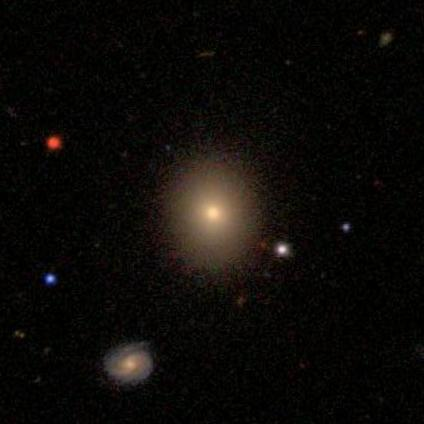
\includegraphics[width=\linewidth]{Figures/Wrongly_Classified/Lenticular/41950.jpg}
    \caption{}
    \label{fig:incorrect_2}
    \end{subfigure}
    \begin{subfigure}[t]{0.23\linewidth}
    \centering
    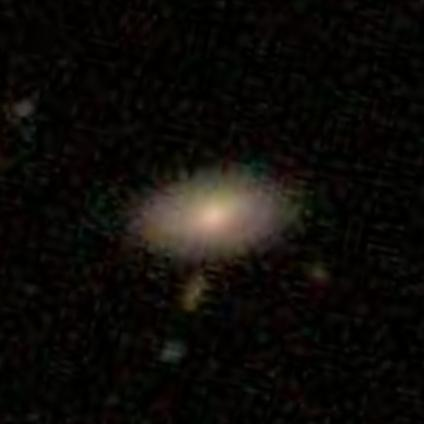
\includegraphics[width=\linewidth]{Figures/Wrongly_Classified/Spiral/13002.jpg}
    \caption{}
    \label{fig:incorrect_3}
    \end{subfigure}
    \begin{subfigure}[t]{0.23\linewidth}
    \centering
    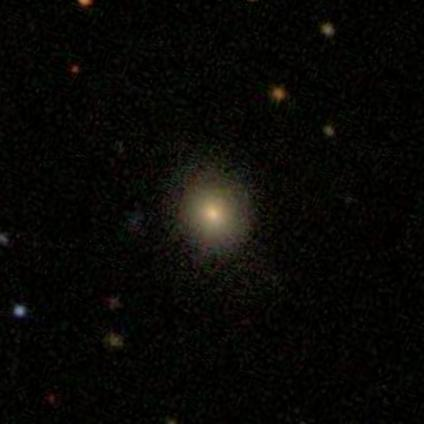
\includegraphics[width=\linewidth]{Figures/Wrongly_Classified/Elliptical/227447.jpg}
    \caption{}
    \label{fig:incorrect_4}
    \end{subfigure}
    
    \caption{A sample of four incorrectly classified images from the Galaxy Zoo 2 sample \citep{Willett2013}. Figures \ref{fig:incorrect_1} and \ref{fig:incorrect_2} show two galaxies classified as Lenticulars by the network but classified as Ellipticals by GZ2. Figure \ref{fig:incorrect_3} shows a galaxy classified as a Spiral by the network but classified as an Elliptical by GZ2. Figure \ref{fig:incorrect_4} shows a galaxy classified as an Elliptical by the network but classified as a Spiral by GZ2. }
    \label{fig:incorrectly_classified}
\end{figure}

In Figure \ref{fig:correctly_classified} it is clear why the network classified each of these galaxies correctly, as the Spirals both have distinct, well defined arms, and the Ellipticals have a smooth surface brightness and ellipsoid shape. 

The first two galaxies in Figure \ref{fig:incorrectly_classified} are good examples of where the network has classified the galaxies as Lenticulars, while the GZ2 classifications are not explicit in its specific class. When assigning classes based off the vote fractions from volunteers, the GZ2 researchers applied an abbreviated class that corresponds to the class from the vote fractions. Although at first thought to match up to the Hubble classification system, where the prefix E corresponds to Elliptical, this is simply a convenient shorthand \citep{Willett2013}. So a smooth galaxy is given the prefix E, and a galaxy with features or disk is given S as a prefix. This means that Lenticulars, which are defined as disk-like in shape, but with no spiral structure, can be given the prefix of either E or S depending on how the volunteers answer the questions. When I binarised the GZ2 data there were no Lenticular galaxies present, as from the GZ2 classifications it is almost impossible to discern which are Lenticulars from just the given classification. 

Figure \ref{fig:incorrect_3} is an Elliptical galaxy incorrectly classified as a Spiral galaxy by the network, one of many that was done so. This fault could be down to the network not having a high enough familiarity with the data as well as the presence of more empty space around each galaxy relative to the images in the NA10 or EFIGI datasets. I believe that fine-tuning the network on the GZ2 dataset could circumvent this problem, as well as cropping the GZ2 images. 

Figure \ref{fig:incorrect_4} is an example of where the networks prediction is perhaps closer to the true classification than the one given by GZ2. Classified as an Elliptical by the network, this received the GZ2 class of Sc, meaning a galaxy with features or a disk and a small noticeable bulge, however this galaxy can easily be seen as an Elliptical. Due to the accuracy of the network, this could be just another incorrect classification and because of the accuracy, it is not possible to say that the network is adept at highlighting incorrect classifications.

\section{Physical Properties of the Sample} \label{sec:physical_prop}
Knowing the morphology of galaxies is very useful when building catalogues to better understand the evolution of these morphologies over time. However, understanding how these morphologies divide galaxies with relation to their physical properties is also essential. In the following section I will discuss the redshifts, Star Formation Rates (SFRs) and the velocity dispersion with relation to the stellar mass of the galaxy, and then present plots of these properties for both true and predicted classifications. The true classifications will come from the NA10 dataset, and the predicted classifications from the highest performing network applied to the GZ2 dataset. The data on each of the properties comes from MPA-JHU measurements released in SDSS DR8. The plots in Figure \ref{fig:y} will be used as a way of comparing the predictions to actual data. \\

\begin{figure}

    \begin{subfigure}[t]{0.499\linewidth}
    \centering
        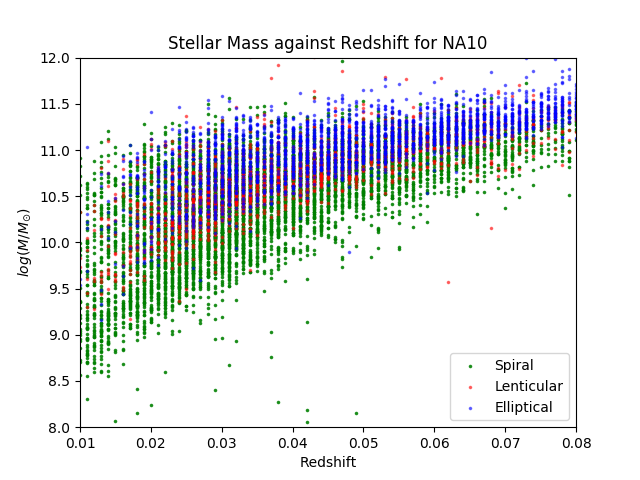
\includegraphics[width=.85\linewidth]{Figures/property_graphs/z_NA10.png}
        \caption{}
        \label{fig:z_na}
    \end{subfigure}
    \begin{subfigure}[t]{0.499\linewidth}
    \centering
        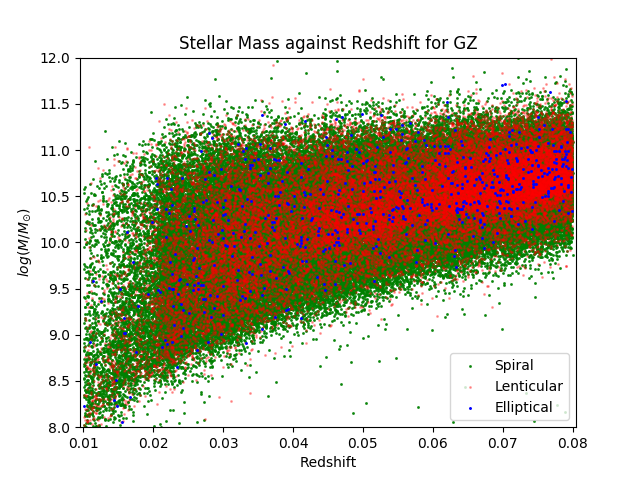
\includegraphics[width=.85\linewidth]{Figures/property_graphs/z_GZ_2.png}
        \caption{}
        \label{fig:z_gz}
    \end{subfigure}
    \begin{subfigure}[t]{0.499\linewidth}
    \centering
        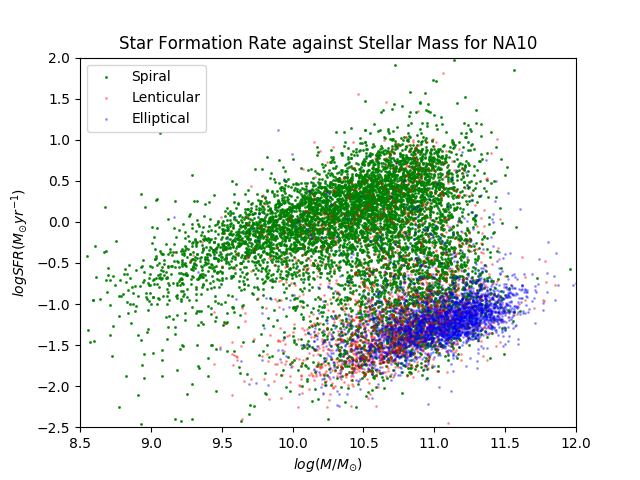
\includegraphics[width=.85\linewidth]{Figures/property_graphs/SFR_NA10.png}
        \caption{}
        \label{fig:sfr_na}
    \end{subfigure}
    \begin{subfigure}[t]{0.499\linewidth}
    \centering
        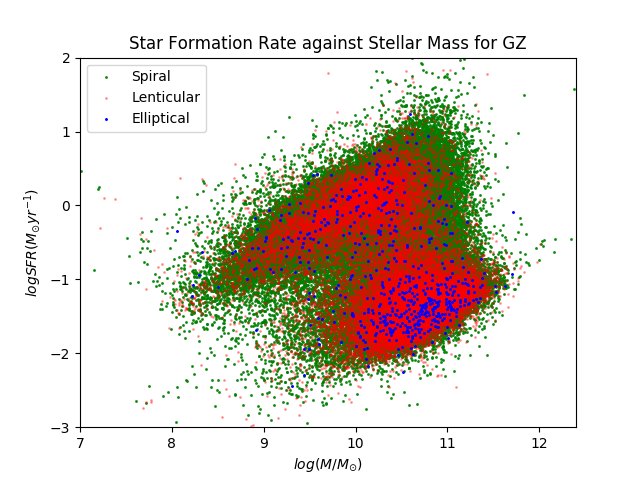
\includegraphics[width=.85\linewidth]{Figures/property_graphs/SFR_GZ_2.png}
        \caption{}
        \label{fig:sfr_gz}
    \end{subfigure}
    \begin{subfigure}[t]{0.499\linewidth}
    \centering
        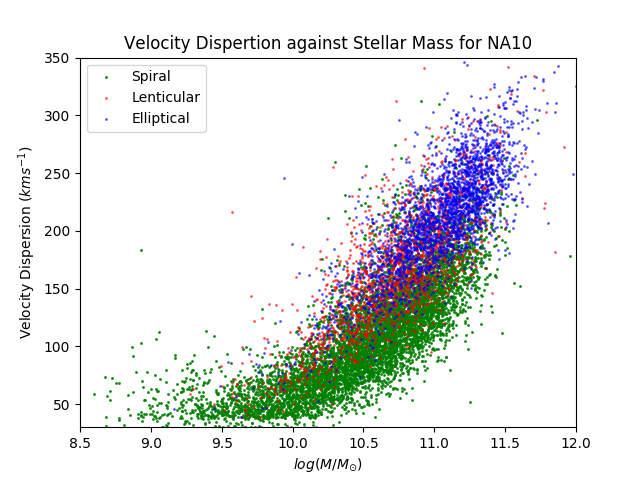
\includegraphics[width=.85\linewidth]{Figures/property_graphs/V_Disp_NA10.png}
        \caption{}
        \label{fig:vdisp_na}
    \end{subfigure}
    \begin{subfigure}[t]{0.499\linewidth}
    \centering
        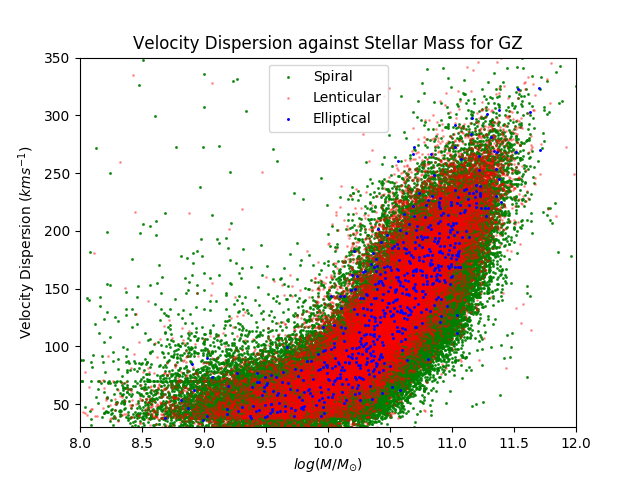
\includegraphics[width=.85\linewidth]{Figures/property_graphs/V_Disp_GZ_2.png}
        \caption{}
        \label{fig:vdisp_gz}
    \end{subfigure}
    \caption{In the left hand columns the physical property plots for the NA10 dataset are presented, and in the right hand columns the same plots for GZ2 are shown. The graphs (a) and (b) are plots of stellar mass against redshift, (c) and (d) are plots of star formation rate against stellar mass and (e) and (f) are plots of velocity dispersion against stellar mass. In each graph the galaxies are split by morphology, clearly shown in each legend. }
    \label{fig:y}
\end{figure}

The redshift is a measure of the Doppler shift in the observed spectral lines of the galaxy, which due to the expansion of the Universe can be converted to lookback time, with a higher redshift being equivalent to further back in time. When the stellar mass is plotted against this quantity, it is possible to distinguish between the different morphologies of galaxies due to the time of their formations and their evolution. As demonstrated in Figure \ref{fig:z_na}, ‘early-type’ galaxies (Elliptical and Lenticular) are found in their highest number densities at larger redshifts, while Spiral, or ‘late-type’, galaxies are found in higher densities at lower redshifts. This agrees with the theory that Spiral galaxies are found at higher densities at lower redshifts, in comparison to Elliptical and Lenticular galaxies. This could be attributed to the evolution of galaxies throughout the lifetime of the Universe however, in \cite{2009MNRAS.393.1324B}, they argue that this could be down to resolution effects for galaxies at a higher redshift.

Figure \ref{fig:z_gz} shows the same plot but with the galaxies split by predicted classification from the GZ2 dataset. It is clear that far more ellipticals and lenticulars are present within this dataset, however they still show that the ‘early-type’ galaxies are present in higher densities at higher redshifts, whilst ‘late-type’ galaxies have what appears to be an almost constant density over the redshift range. \\

The star formation rate (SFR) is the total mass of stars formed per unit time by a galaxy and is a useful quantity towards understanding the formation and evolution of galaxies \citep{fundamentals_book}. As demonstrated clearly in Figure \ref{fig:sfr_na}, galaxies are split by their morphology when their SFR is plotted against their stellar mass. Ellipticals and Lenticulars tend to have a lower SFRs than Spiral galaxies \citep{2011IAUS..270..335G}, and through the study of their stars it is understood that there was and early and intense period of star formation which then then quickly stopped. This observed reduction in the SFR is thought to partly be from the galaxy using up the gas for star formation, but also from quenching processes that remove the gas from the galaxy \citep{2014MNRAS.440..889S}.

For Spiral galaxies the SFR is typically higher than in Ellipticals and within the galaxy itself, it is found that the SFR is usually higher in the arms \citep{2010ApJ...725..534F}, potentially due to the spiral arms collecting gas in higher densities in these areas. The SFR of these galaxies can be affected by processes such as stellar feedback and AGN, which eject gas from the galaxy. The SFR can also be affected by mergers, which have been shown to increase the SFR, although only by small amounts \citep{2019A&A...631A..51P}. 

In Figure \ref{fig:sfr_na} this distinction between the morphologies is present, with Spiral galaxies occupying a higher SFR relative to their stellar mass and Elliptical and Lenticular galaxies generally having lower SFRs. 

Figure \ref{fig:sfr_gz} on the other hand does not exhibit this distinction as clearly, with the predicted Lenticular galaxies occupying higher SFRs than are expected. This can be attributed to the low accuracy in the network and the clear bias towards giving galaxies a Lenticular classification explained in Section \ref{sec:classified_images}. \\

The next property presented here is the velocity dispersion, a value quantifying the statistical dispersion of the velocity about the mean velocity. This property is an important one to measure as this value varies when looking at the processes that quench or increase star formation \citep{2012ApJ...760...62B}. The velocity dispersion also relates very well to mass in both Spiral (Tully-Fisher Relation) and Elliptical (Faber-Jackson relation) galaxies. These relations show linearity between the Mass and velocity dispersion of the galaxy, so higher mass galaxies tend to have a higher velocity dispersion for all morphologies present.

The plot of galaxies with classifications from the NA10 dataset in Figure \ref{fig:vdisp_na} shows a clear separation of morphologies, with Spiral galaxies occupying lower velocity dispersions and Elliptical and Lenticular galaxies having higher velocity dispersions on average. 

However this relation is not upheld in the data plotted in Figure \ref{fig:vdisp_gz}, as there is no clear morphological split between the ‘early’ and ‘late’ type galaxies, showing again the bias of the network to predict a galaxy as a Lenticular. 



\section{Conclusions and Further Work} \label{sec:conc}
\subsection{Conclusions}
In this report I demonstrate how a combination of transfer learning and specific methods of fine-tuning can improve the accuracy and generalisation of a convolutional neural network when applied to the task of classifying galaxies based on their morphology. This reduction in the size of the training dataset allows for analysis of more specific features like the number of spiral arms, the presence of a bulge, rings, bars and lenses, all of which have small datasets to be trained upon. This also means that when future surveys begin to release data, new networks do not have to be trained from scratch as networks applied to previous surveys can be reused and simply fine-tuned to this specific data release. Crucially, this will reduce the time that it takes to release catalogues of morphologies for the data, as extensive visual classifications will not be necessary for the fine-tuning of the pre-trained network. \\

I took data from the fashion\_MNIST and Nair \& Abraham (NA10) datasets to pre-train 3 networks each, all with the same architecture and hyperparameters. I then applied two different forms of fine-tuning (allowing the network to train specific layers on the target data) to two of those networks for each dataset. In one test I only fine-tuned the dense classifying layers, and in the other I fine-tuned the final two convolutional layers as well as the dense layers. A small training set from the EFIGI dataset was used for fine-tuning. All six of these networks were then applied to the testing sample from EFIGI. The networks were all trained in a way such that they produced 3 probabilities for each morphology in the data, Lenticular, Elliptical and Spiral galaxies.  A network trained on just the EFIGI training sample was used as a baseline to compare how the transfer learning affected the final performance of the networks. For all 7 of these networks Receiver Operating Characteristic curves were produced in order to directly compare how they performed, as well as analyse how they performed on each class within the dataset. 

I also applied the highest performing network to the Galaxy Zoo 2 (GZ2) sample of 118000 images and further investigated how my network performed by comparing the graphs of physical properties produced using those predictions against the graphs of properties from the NA10 sample with the correct classes. \\

My results showed that a combination of pre-training on the NA10 dataset and fine-tuning the final two convolutional layers as well as the dense classifying layers produced the best results, with an accuracy of $93.6\%$. When compared against the network trained on just the EFIGI training sample, transfer learning was shown to only be effective when some form of fine-tuning takes place, as the networks pre-trained on the fashion\_MNIST and NA10 datasets and the applied to the EFIGI sample without fine-tuning performed worse than the network simply trained on EFIGI. This aligns with the theory, as networks trained on other samples of data are not familiar with the EFIGI images so will not perform as well on them.

When comparing the two methods of fine-tuning, training just the dense layers produced worse results than if trained on the final two convolutional layers as well as the dense layers. This can be attributed to how the final two convolutional layers extract higher level features from images, so it is at these layers that the differences between the NA10 and EFIGI images are distinct. By fine-tuning these layers as well as the dense ones the network is familiar with the specific scale and colours of the EFIGI galaxies and can identify high level features more effectively. 

I also found that the network pre-trained on the fashion\_MNIST images performed poorly in comparison to the baseline network and the NA10 networks, demonstrating that a network pre-trained on data that is dissimilar to the target sample will not perform as well as pre-training on images similar to the target, galaxies in this case.

My results also highlighted the difficulties the networks faced when classifying Lenticular galaxies, as across all networks they were the class with the highest rate of incorrect classifications. This could be due to how they are the transition class between the two extreme Elliptical and Spiral classes, so the network struggled to place Lenticular galaxies in the middle class at times. \\

From plotting the graphs of the physical properties of the galaxies within the sample, it is clear that when applied to new data the network is still lacking in generalisation as it seemed to over classify Lenticular galaxies, and only reached an accuracy of $45\%$. Although there were some instances where the network seemed to classify more accurately in comparison to the class given by the GZ2 catalogue, this cannot be seen as a trend due to the networks low accuracy and potential random nature of how it classified.

From the graphs of the physical properties the faults of the network are clear, for example in the plot of SFR against stellar mass, the predicted Lenticular galaxies occupy the same space as those predicted as Spiral galaxies. This is incorrect as Lenticular galaxies are expected to have a lower SFR for a given mass in comparison to Spirals as they are mostly had an intense period of star formation early in their lives, and then evolved into the galaxies present in the redshifts observed in our sample.\\

\subsection{Further Work}
For further work I would like to investigate how these methods of pre-training and fine-tuning can be applied to the more specific features mentioned above, and secondly if a robust catalogue of galaxies with the probabilities of these specific features being present could be produced. In order to do this I would take advantage of the Galaxy Zoo project and the extensive catalogue of vote fractions for all the questions in the decisions tree that volunteers go through to train the network and compare against. Future surveys will be releasing data that would take over 5 years to classify based off the current Galaxy Zoo method, so having neural networks that can highlight these more specific features and achieve high accuracies when fine-tuned on a small sample will be invaluable in reducing the time needed to classify galaxies.\\

Another way that scientists can prepare networks for future surveys is by training on data that is similar to future data releases in how it is processed. As shown in Section \ref{sec:classified_images}, slight differences in scale and colour of the galaxy in the image can have detrimental effects to the accuracy of the network. So by using data from surveys like the Hyper Suprime-Cam Subaru Strategic Survey \citep{2018PASJ...70S...8A}, which has processed the data using the same pipeline as the Large Synoptic Survey Telescope (LSST), it would be possible to pre-train a network on images that would be close to data from future LSST data releases. \\

Although the use of fashion\_MNIST data to pre-train the network was not successful in this project, I would be interested in investigating how data with features similar to that of galaxies would perform when transferring knowledge. When classifying the number of arms in a Spiral galaxy a good pre-training sample could be images of hurricanes from the American National Hurricane Center as they have that spiral shape that could transfer well across the galaxy data. 


\newpage
\section*{Acknowledgements} 
I would like to thank my supervisor, Dr Brooke Simmons, for her help and support during this project. I will also like to thank Sam Dicker for his help with coding, as well as Pablo Bilbao, Charlie Steward and George Ridgard for assistance with proofreading. This project would not have been possible without the \verb|Keras| neural network API that is built on top of \verb|Tensorflow|, so thank you to the creators, Fran\c{c}ois Chollet et al.



\bibliography{references.bib} 
\end{document}
